\documentclass[11pt,twocolumn,a4paper]{article}

% ---------- Packages ----------
\usepackage{graphicx}
\usepackage{enumitem}
\usepackage{geometry}
\usepackage{fancyhdr}
\usepackage[dvipsnames]{xcolor}
\usepackage{tcolorbox}
\usepackage{titlesec}
\usepackage{lastpage}
\usepackage{amsmath,amssymb,amsfonts}
\usepackage{booktabs,multirow,tabularx,array}
% \usepackage{tikz}
% \usetikzlibrary{arrows.meta,positioning,fit,calc,shapes.geometric,backgrounds}
\usepackage{cite}
\usepackage{microtype}
\usepackage{float}
\usepackage{abstract}
\usepackage{balance}
\usepackage{dblfloatfix}
\usepackage{url}

% ---------- Hyperlinks ----------
\usepackage[
    colorlinks=true,
    allcolors=blue,
    pdfborder={0 0 1}
]{hyperref}

% ---------- Custom Commands ----------
\newcommand{\appname}{\textsc{AI Conference Research Observatory}}
\newcommand{\datasetname}{\textsc{NeurIPS-39}}
% System name used throughout the paper. Rename here to rebrand everywhere.
\newcommand{\method}{\textsc{BadmintonMine}}

% ---------- Colors ----------
\definecolor{NavyHead}{RGB}{24,50,82}
\definecolor{SteelSub}{RGB}{58,86,120}
\definecolor{DarkRed}{RGB}{140,45,45}
\definecolor{SoftCoral}{RGB}{214,104,83}
\definecolor{CreamBox}{RGB}{255,249,237}

% ---------- Page Geometry ----------
\geometry{
    a4paper,
    margin=0.65in,
    columnsep=0.25in
}

% ---------- Paragraph and List Formatting ----------
\setlength{\parindent}{0pt}
\setlength{\parskip}{0.35em}
\setlist[itemize]{leftmargin=1.2em,itemsep=0.1em,topsep=0.15em}
\setlist[enumerate]{leftmargin=1.4em,itemsep=0.1em,topsep=0.15em}
\renewcommand{\arraystretch}{1.12}

% ---------- Abstract Formatting ----------
\renewcommand{\abstractnamefont}{\normalfont\large\bfseries}
\renewcommand{\abstracttextfont}{\normalfont\small}
\setlength{\absleftindent}{0pt}
\setlength{\absrightindent}{0pt}

% ---------- Section Formatting ----------
\titleformat{\section}
  {\color{NavyHead}\large\bfseries}
  {\thesection.}{0.5em}{}
  [{\vspace{-3pt}\color{DarkRed}\rule{\columnwidth}{0.8pt}}]
\titleformat{\subsection}
  {\color{SteelSub}\normalsize\bfseries}
  {\thesubsection.}{0.5em}{}
\titlespacing{\section}{0pt}{0.7em}{0.35em}
\titlespacing{\subsection}{0pt}{0.55em}{0.2em}

% ---------- Header/Footer ----------
\newcommand{\VinLogo}{
\includegraphics[scale=0.11]{figures/VinUni_logo.png}}
\newcommand{\CommonFooter}{
    \fancyfoot[L]{COMP4040 Data Mining and Big Data Analytics}
    \fancyfoot[C]{}
    \fancyfoot[R]{\thepage/\pageref{LastPage}}
}

\pagestyle{fancy}
\fancyhf{}
\fancyhead[L]{\VinLogo}
\fancyhead[R]{\footnotesize College of Engineering and Computer Science \\ VinUniversity, Hanoi, Vietnam}
\CommonFooter
\renewcommand{\headrulewidth}{0.4pt}
\renewcommand{\footrulewidth}{0.4pt}

\fancypagestyle{firstpage}{
    \fancyhf{}
    \fancyhead[L]{\VinLogo}
    \fancyhead[R]{\footnotesize College of Engineering and Computer Science \\ VinUniversity, Hanoi, Vietnam}
    \CommonFooter
    \renewcommand{\headrulewidth}{0.4pt}
    \renewcommand{\footrulewidth}{0.4pt}
}

% ---------- Title ----------
\title{\bfseries\LARGE An Integrated Badminton Analytics and
\\ Data-Mining Pipeline}

\author{\normalsize
\bf Cao Pham Minh Dang, Pham Dinh Hieu, Pham Minh Hieu \\[0.2em]
\small College of Engineering and Computer Science, VinUniversity, Vietnam\\
\texttt{\{24dang.cpm, 24hieu.pd, 22hieu.pm\}@vinuni.edu.vn} \\
\small Github Repository: \href{https://github.com/minhdang050806/COMP4040--Badminton-Match-Analysis}{Link} \quad
}
\date{}

\begin{document}

\twocolumn[
\maketitle
\thispagestyle{firstpage}

\begin{abstract}    
Badminton broadcasts encode rich tactical information---stroke choices, rally
structure, and player movement---yet this information exists as pixels rather
than structured data. Recovering it requires a multi-stage perception chain:
isolating rally footage, tracking the shuttle, localizing both players,
identifying hit moments, and classifying fine-grained stroke types into ordered
rally sequences, where errors at any stage can corrupt downstream tactical
analysis. We present \method, an integrated badminton video analytics and
data-mining pipeline that couples SA-CNN rally filtering, TrackNetV3 shuttle
tracking, YOLO-pose player extraction, court normalization, and a fine-tuned
Badminton-Stroke Transformer. This output feeds five tactical mining analyses:
stroke composition, Markov transitions, frequent motif discovery, movement
profiling, and strategy clustering. Evaluated on unseen ShuttleSet videos~41--44,
the system yields 3{,}178 evaluated stroke predictions at 69.04\% side-aware
top-1 accuracy and 66.64\% macro-F1. The key result is that \emph{sequence
coherence} matters more than per-stroke accuracy for mining: reducing the
predicted \textit{none} rate from 56.43\% to 6.70\% lowers transition-matrix
error and recovers a coherent attack--defence grammar around net shots, lifts,
smashes, and defensive replies. Crucially, we validate the \emph{mining}, not
just the perception: running every analysis on matched ground-truth labels for
the same events shows that predicted composition (KL $0.04$), motif rankings
(Spearman $0.66$), and transition structure (Frobenius $1.23$, below unigram and
random baselines) all track the truth, while clustering is faithful at the
feature level ($\bar{r}=0.79$) but only descriptive at the assignment level
(ARI $0.17$). Our analyses provide intuitive match-level summaries, shot-response
tendencies, recurring tactical phrases, spatial movement patterns, and
high-level strategy groupings.
\footnote{Code repository: \url{https://github.com/minhdang050806/COMP4040--Badminton-Match-Analysis}}
\end{abstract}

\vspace{0.8em}
]

Badminton is a fast-paced racket sport in which rally dynamics can shift within
a handful of exchanges. Coaches and analysts regularly pose questions such as
which strokes dominate a match, what replies tend to follow a smash, whether
forward movement correlates with attacking opportunities, and whether opposing
players exhibit distinct tactical profiles. These are data-mining questions, yet
broadcast video does not supply the structured event tables needed to answer
them. The raw signal must be converted from pixels into an ordered stroke
sequence, and that conversion requires a chain of perception models whose errors
accumulate before any mining step begins.

This conversion is technically demanding. The shuttlecock is small and often
motion-blurred; broadcast footage interleaves replays, close-ups, scoreboard
inserts, and non-rally segments that must be filtered out. The far-court player
appears at low resolution and may be partially occluded, degrading pose estimates
at exactly the positions where attacking strokes are most frequent. Stroke
classification is further complicated by the fine-grained taxonomy of badminton
labels: a reliable system must distinguish, for example, a net shot from a return
net, a drop from a push, or a smash from closely related attacking strokes.
Without accounting for this error propagation, tactical analyses risk drawing
conclusions from a corrupted event stream.

We construct and evaluate \method, a practical end-to-end pipeline that converts
badminton broadcast video into mineable tactical data. The overall architecture
is depicted in Figure~\ref{fig:workflow}. The central research question is:
\emph{\textbf{Can an integrated raw-video pipeline recover badminton stroke sequences
that are sufficiently accurate and continuous to support meaningful tactical
mining on unseen matches?}}  Our answer is cautiously affirmative: by combining
simple yet reliable perception modules with careful integration, we recover
coherent stroke sequences that support a variety of interpretable analyses.

It is important to state the scope of this benchmark. The pipeline processes
unseen raw frames through rally filtering, shuttle tracking, pose extraction,
feature construction, stroke classification, and tactical mining. It does not
yet constitute a fully automatic system for arbitrary unlabeled broadcasts: the
unseen-video benchmark relies on ShuttleSet hit-frame indices to construct
stroke windows and on ShuttleSet homographies for court normalization. We make
this boundary explicit because it defines what the reported metrics demonstrate,
and because the primary bottleneck we identify—far-side player extraction—remains
an open problem even under fully automatic setups.

Our main contributions are:
\begin{itemize}[leftmargin=*,nosep]
  \item an integrated raw-video badminton pipeline linking rally filtering,
  shuttle tracking, pose extraction, and stroke classification into a single
  reproducible workflow;
  \item five tactical-mining analyses—stroke composition, Markov transitions,
  frequent motifs, movement profiling, and clustering—that illustrate how the
  recovered event stream can support diverse insights;
  \item a mining-validation protocol that re-runs every analysis on matched
  ground-truth labels and reports the predicted-vs-true gap for each view
  (distribution KL/$\chi^2$, motif rank correlation, transition baselines, and
  cluster ARI), turning unverified tactical claims into measured ones.
\end{itemize}

\begin{figure*}[t]
  \centering
  \includegraphics[width=\textwidth]{images/Overall_workflow.png}
  \caption{\textbf{End-to-end \method{} pipeline.} Raw broadcast frames are
  processed through rally filtering, shuttle tracking, player pose extraction,
  and stroke classification. The resulting structured stroke table drives all
  five tactical mining analyses. In our benchmark, ShuttleSet hit-frame labels
  and homographies are supplied for window construction and court normalization.}
  \label{fig:workflow}
\end{figure*}


%-----------------------------------------------------------------------
\section{Related Work}
%-----------------------------------------------------------------------

\paragraph{Badminton datasets.}  ShuttleSet provides broadcast videos, set-level
annotations, stroke labels, homography information, and pre-extracted features
for badminton analysis \cite{shuttleset}. Its paired structure—raw video
alongside structured labels—makes it well suited to evaluating how much tactical
information survives end-to-end prediction from video. BadmintonDB focuses on
player-specific match analysis and outcome prediction \cite{badmintondb}.
Recently, the FineBadminton project introduced a large-scale dataset with a
multi-level annotation hierarchy ranging from low-level actions to decision
evaluation \cite{finebadminton}. The dataset and associated FBBench benchmark
are designed to challenge multimodal models on nuanced spatio-temporal reasoning,
but their focus is on higher-level semantics rather than fine-grained stroke
classification. We adopt ShuttleSet as our primary benchmark because its
annotations support evaluation at the stroke, rally, and sequence levels
simultaneously.

\paragraph{Rally filtering, shuttle tracking, and hit detection.}
Rally filtering separates playable footage from non-rally broadcast segments, a
prerequisite for any downstream processing. Shuttle tracking is typically
formulated as frame-level heatmap or coordinate prediction; TrackNetV2
introduced an efficient network architecture for this task in badminton video
\cite{tracknetv2}, and we build on a TrackNetV3 implementation for coordinate
extraction and denoising. Hitting-event detection has been studied directly
using specialized models \cite{chen2023hitting}. Recent work has also proposed
refining shuttle hit times by combining TrackNet trajectory predictions with
swing detection from YOLOv7 \cite{hsu2024enhancing}, improving shot extraction
in monocular-camera settings. In the present work, exact ShuttleSet hit-frame
labels define the unseen-video benchmark; trajectory-based hit detection
remains the prerequisite step for fully unlabeled deployment.

\paragraph{Pose estimation and stroke classification.}
Player pose provides body keypoints and on-court position, both of which are
necessary inputs to stroke classification. MMPose is a widely used
pose-estimation toolbox \cite{mmpose}; our pipeline employs a YOLO-pose
checkpoint for efficient per-window feature extraction. For stroke recognition,
the Badminton-Stroke Transformer (BST) models racket-sport strokes jointly from
player skeletons, positions, and shuttle kinematics \cite{chang2025bst}.
We fine-tune the \texttt{BST\_CG\_AP} variant as the final stroke classifier.

\paragraph{Sports tactic mining and immersive analysis.}
Tactical analysis from structured event sequences is an established area in
sports analytics. Stroke distributions characterize match composition,
transition matrices encode sequential stroke tendencies, and frequent-sequence
mining identifies recurring tactical phrases \cite{shuttleset}. Movement
profiling connects spatial displacement with stroke selection. KMeans clustering
\cite{kmeans} paired with silhouette analysis \cite{silhouette} offers a
standard approach for profile summarization, but cluster validity must be
confirmed through stability tests rather than visual inspection alone. Beyond
batch analysis, immersive systems such as VIRD provide interactive 3D visual
analytics for coaches and players by reconstructing rally scenes in virtual
reality \cite{vird2023}. Our work differs by focusing on automated recovery of
stroke sequences from raw video and on producing interpretable mining outputs
from predicted event streams rather than on visualization tools.

\paragraph{Positioning \method{} against prior work.}
Table~\ref{tab:comparison} summarises how \method{} sits relative to the
systems above across five dimensions: input modality, output, degree of
automation, support for tactical mining, and evaluation protocol. No prior
system simultaneously takes raw video as input, produces a structured stroke
event stream, \emph{and} validates the downstream mining against ground truth.
TrackNet-based systems handle the video-to-trajectory step but stop at shuttle
coordinates. BST handles stroke classification but requires pre-extracted
features, not raw frames. ShuttleSet's own analysis tools operate on
ground-truth annotations rather than predicted events, providing an upper bound
but not an end-to-end pipeline. VIRD delivers immersive visualisation but
relies on structured input and does not address recovery from raw video.
\method{} fills the gap between raw video and a validated tactical analysis by
chaining these components and measuring how much tactical signal survives
end-to-end prediction.

\begin{table*}[t]
  \caption{Qualitative comparison of related badminton analytics systems.
  ``Partial'' automation means the system processes raw video for some stages
  but relies on supplied metadata (hit-frame indices or homographies) for
  others.}
  \label{tab:comparison}
  \centering
  \small
  \setlength{\tabcolsep}{4pt}
  \renewcommand{\arraystretch}{1.15}
  \begin{tabular}{p{2.8cm} p{3.2cm} p{2.8cm} p{1.6cm} p{1.6cm} p{3.5cm}}
    \toprule
    System & Input & Output & Fully auto? & Tactical mining? & Evaluation \\
    \midrule
    ShuttleSet analysis \cite{shuttleset}
      & Ground-truth stroke annotations
      & Tactical statistics
      & No
      & Yes
      & Annotation-derived; no pred-vs-truth gap \\[3pt]

    BST \cite{chang2025bst}
      & Pre-extracted features (pose, shuttle)
      & Stroke class per window
      & No
      & No
      & Classification accuracy on held-out clips \\[3pt]

    TrackNet-based systems \cite{tracknetv2,hsu2024enhancing}
      & Raw broadcast video
      & Shuttle trajectory; hit-frame cues
      & Partial
      & No
      & Tracking coverage; hit-detection F1 \\[3pt]

    VIRD \cite{vird2023}
      & Structured / visual input
      & Interactive 3-D VR visualisation
      & No
      & Visualisation only
      & User study / visual inspection \\[3pt]

    \textbf{\method{} (ours)}
      & Raw video + supplied hit indices \& homographies
      & Stroke event stream + five mining analyses
      & Partial
      & Yes
      & Pred-vs-truth mining validation (KL, Frobenius, Spearman, ARI) \\
    \bottomrule
  \end{tabular}
\end{table*}

%-----------------------------------------------------------------------
\section{Dataset and Preprocessing}
%-----------------------------------------------------------------------

\subsection{Source and Scale}

Our experiments use ShuttleSet, a badminton broadcast dataset with stroke-level
annotations. Table~\ref{tab:data} summarizes the local snapshot: 44 raw
broadcast videos, 104 set annotation files, 36{,}482 annotated strokes, and
3{,}683 annotated rallies, along with six pre-extracted feature variants
comprising 33{,}481 prepared clips each. The active BST feature variant employs
a fixed sequence length of 100 frames. Videos~1--40 are reserved for
development; videos~41--44 form the held-out evaluation set used throughout
this work. While newer datasets such as FineBadminton provide richer semantic
annotations \cite{finebadminton}, ShuttleSet remains the only public resource
with aligned hit-frame indices, homography parameters, and stroke-level labels
required for our pipeline.

\begin{table}[t]
  \caption{Local ShuttleSet snapshot and data split used for evaluation.}
  \label{tab:data}
  \centering
  \small
  \begin{tabular}{lr}
    \toprule
    Item & Count or split \\
    \midrule
    Raw broadcast videos & 44 \\
    Set annotation files & 104 \\
    Annotated strokes    & 36{,}482 \\
    Annotated rallies    & 3{,}683 \\
    Prepared clips per variant & 33{,}481 \\
    Training videos      & 1--40 (train split) \\
    Validation videos    & 1--40 (val split, model selection only) \\
    Unseen evaluation    & 41--44 (held-out, never seen during training) \\
    Clean unseen predictions & 3{,}178 \\
    \bottomrule
  \end{tabular}
\end{table}

\subsection{Data Splits and Evaluation Protocol}
\label{sec:splits}

All 44 videos originate from ShuttleSet's pre-defined splits.
Videos~1--40 provide the \textbf{training set} (25{,}741 clips) and
\textbf{validation set} (4{,}241 clips); the validation set is used
\emph{only} for model selection---early stopping halted training at
epoch~6 based on validation macro-F1.
Videos~41--44 form the \textbf{held-out test set} (3{,}499 collated
clips; 3{,}178 clean primary events after removing feature-alias
duplicates). These four matches were withheld from all training, tuning,
and threshold decisions and evaluated exactly once to produce the figures
reported throughout this paper.

\subsection{Annotations and Label Preparation}

Table~\ref{tab:annotation_layers} summarizes the annotation layers used by the
pipeline. These annotations provide the temporal, spatial, and identity
information needed to convert raw video into ordered stroke-level examples.

\begin{table*}[h]
  \caption{Annotation layers used for feature construction, evaluation, and tactical mining.}
  \label{tab:annotation_layers}
  \centering
  \small
  \begin{tabular}{p{3.2cm} p{5.3cm} p{4.4cm}}
    \toprule
    Annotation layer & What it records & Role in the pipeline \\
    \midrule
    Stroke labels
      & Hitter side and stroke type for each event
      & Defines the supervised classification target \\[3pt]

    Rally identifiers
      & Rally ID and event order within each rally
      & Builds ordered stroke sequences for transitions and motifs \\[3pt]

    Hit-frame indices
      & Video frame where each stroke occurs
      & Anchors fixed-length stroke windows in raw video time \\[3pt]

    Homography parameters
      & Mapping from image coordinates to normalized court coordinates
      & Supports court normalization and movement profiling \\[3pt]

    Player identities
      & Persistent player information from ShuttleSet metadata
      & Used for evaluation and player-level movement analysis \\
    \bottomrule
  \end{tabular}
\end{table*}

The classification target contains 25 side-aware classes: one background
\texttt{none} class, 12 Top-side stroke classes, and 12 Bottom-side stroke
classes. Here, \emph{Top} and \emph{Bottom} are camera-relative sides, not
persistent player identities. For example, a Top-side smash means that the
far-court player, as seen by the broadcast camera, performed a smash.

\subsection{Preprocessing Pipeline}

Raw broadcasts are converted into aligned stroke windows through four sequential
stages, summarised in Table~\ref{tab:preproc}. Rally filtering identifies active
play segments and discards non-rally footage. Shuttle tracking predicts
frame-level coordinates, suppresses implausible jumps, and fills short gaps.
Window construction extracts a fixed-length frame range around each hit-frame,
and pose extraction obtains body keypoints and positions for both players. Each
stroke window includes four feature streams (player keypoints, positions,
shuttle coordinates, and validity masks) that feed the stroke classifier.

\begin{table*}[h]
  \caption{Preprocessing stages with corresponding operations and outputs.}
  \label{tab:preproc}
  \centering
  \small
  \begin{tabular}{p{3.3cm} p{5.5cm} p{4.1cm}}
    \toprule
    Stage & Operation & Output \\
    \midrule
    Rally filtering
      & Separate rally frames from non-play broadcast segments & Rally frame intervals \\
    Shuttle tracking
      & Predict shuttle coordinates, remove jumps, interpolate gaps & Denoised shuttle positions \\
    Window construction
      & Extract fixed-length frame range around each hit frame & Stroke windows \\
    Pose extraction
      & Extract, order, and normalize player keypoints & Player features and validity masks \\
    \bottomrule
  \end{tabular}
\end{table*}

%-----------------------------------------------------------------------
\section{Modeling}
%-----------------------------------------------------------------------

Table~\ref{tab:components} provides a consolidated summary of key metrics across
the perception stages. Rather than presenting exhaustive implementation details,
we highlight the aspects that most affect downstream analysis.

\begin{table*}[t]
  \caption{Per-stage performance metrics across the \method{} pipeline.}
  \label{tab:components}
  \centering
  \small
  \begin{tabular}{llr}
    \toprule
    Component & Metric & Result \\
    \midrule
    SA-CNN rally filtering & Validation F1 & 0.903 \\
    SA-CNN & Annotated-hit coverage & 97.32\% \\
    TrackNetV3 tracking & Visible-frame coverage (denoised) & 90.99\% \\
    BST classifier & Validation macro-F1 & 0.805 \\
    YOLO-pose features & Top / Bottom pose-valid rate & 54.29\% / 98.96\% \\
    \bottomrule
  \end{tabular}
\end{table*}

\paragraph{Rally Scene Filtering.}
SA-CNN is a binary classifier that separates court-view frames from non-play
footage—score screens, replays, crowd shots. Trained on 20k labelled images, it
achieves an F1 score of 0.903 and retains 97.32\% of annotated hits, ensuring
that shuttle tracking is not run on irrelevant frames.

\paragraph{Shuttle Tracking.}
TrackNetV3 predicts frame-level shuttle coordinates. Post-processing removes
implausible jumps and interpolates short gaps, achieving a denoised visible
coverage of 90.99\%. Representative trajectories are coherent across rally
frames, although some noise near rally boundaries underscores the need for
precise filtering.

\paragraph{Pose Estimation.}
YOLO-pose extracts body keypoints and positions for both players in each window.
Valid keypoints are obtained for 98.96\% of near-side frames, but only 54.29\%
for far-side frames. This asymmetry proves to be the main bottleneck: when the
far-side pose is absent, classification accuracy drops sharply.

\paragraph{Stroke Classification.}
The Badminton-Stroke Transformer (\texttt{BST\_CG\_AP}) is fine-tuned on
ShuttleSet training clips. On the clean unseen set, it achieves 69.04\%
side-aware top-1 accuracy and 66.64\% macro-F1 across 3{,}178 evaluated strokes.
Player-side accuracy reaches 93.05\%, indicating that the model reliably
identifies which side struck the shuttle even when stroke-type distinctions are
confused.  The pipeline’s principal improvement over earlier versions is the
dramatic reduction of \texttt{none} predictions, from 56.43\% to 6.70\%, which
restores sequential coherence and is critical for the mining analyses.

Table~\ref{tab:per_video} breaks down results across the four held-out
matches. Accuracy ranges from 53.3\% (Video~43, Marin vs.\ Chochuwong
SF) to 76.6\% (Video~44, Antonsen vs.\ Axelsen Finals), a 23-point
spread that reflects match-level variation in broadcast angle and
far-side player visibility. The Finals match (Video~44) benefits from
more consistent near-court exchanges, whereas the semi-final
(Video~43) involves more aggressive backcourt play, compounding
far-side pose errors. Video~41 serves as the reference split used for
validation during training; it is included here only for completeness.

\begin{table}[t]
  \caption{Per-video stroke-classification results on the held-out
  unseen set (videos~41--44). Top-3 accuracy counts a prediction
  correct if the true label appears among the model’s three highest
  scoring classes.}
  \label{tab:per_video}
  \centering
  \small
  \begin{tabular}{clrrrr}
    \toprule
    Video & Match (BWF WTF 2020) & $n$ & Top-1 & Top-3 & Macro-F1 \\
    \midrule
    41 & Ng Ka Long vs.\ Srikanth (QF)  & 1{,}151 & 73.7\% & 90.4\% & 0.723 \\
    42 & Sindhu vs.\ Chochuwong (QF)    &   619   & 64.0\% & 85.1\% & 0.612 \\
    43 & Marin vs.\ Chochuwong (SF)     &   550   & 53.3\% & 74.2\% & 0.478 \\
    44 & Antonsen vs.\ Axelsen (Finals) &   858   & 76.6\% & 95.2\% & 0.725 \\
    \midrule
    \textbf{All} & & \textbf{3{,}178} & \textbf{69.0\%} & \textbf{87.9\%} & \textbf{0.664} \\
    \bottomrule
  \end{tabular}
\end{table}

Table~\ref{tab:top_confusions} lists the most frequent stroke-type
confusion pairs on the test set (side-agnostic). The dominant errors
cluster around \emph{net-zone strokes}: net shot is confused with return
net (89 times) and predicted as \texttt{none} (84 times), and lob is
confused with push (93 times). These three pairs alone account for
266~of the 984 total errors. Crucially, net~shot and return~net are
tactically adjacent---both are soft forecourt exchanges---and are
visually similar when the far-side player is absent or blurred.
The smash$\leftrightarrow$drop confusion (55+49) reflects the shared
overhead mechanics and limited shuttle visibility at the contact point.

\begin{table}[t]
  \caption{Top stroke-type confusion pairs on the 3{,}178-event unseen
  set (side-agnostic; \texttt{none} pairs included where notable).
  Each row is one confusion direction; the symmetric counterpart is
  listed separately when it is also a top error.}
  \label{tab:top_confusions}
  \centering
  \small
  \begin{tabular}{llr}
    \toprule
    True stroke & Predicted as & Errors \\
    \midrule
    lob         & push              & 93 \\
    net shot    & return net        & 89 \\
    net shot    & \texttt{none}     & 84 \\
    drop        & smash             & 55 \\
    smash       & drop              & 49 \\
    push        & lob               & 44 \\
    return net  & drive             & 36 \\
    lob         & clear             & 35 \\
    \bottomrule
  \end{tabular}
\end{table}


%-----------------------------------------------------------------------
\section{Tactical Data Mining}
%-----------------------------------------------------------------------

We convert the structured stroke table into five complementary tactical views.
Each view answers a different question: what strokes are used, how strokes
follow one another, which multi-stroke phrases recur, how movement relates to
stroke choice, and whether high-level profiles cluster into interpretable
groups.

A central methodological commitment of this work is that we validate the
\emph{mining}, not only the perception. The same 3{,}178 evaluated events carry
both predicted and ground-truth stroke labels, so every analysis can be run
twice---once on the predicted stream and once on the matched truth---and the
predicted-vs-true gap measured directly. Table~\ref{tab:mining_eval}
consolidates this evaluation: for each task we list its input, algorithm,
metric, a baseline, and the measured conclusion. The remainder of this section
develops each view and its validation in turn.

\begin{table*}[t]
  \caption{\textbf{Data Mining Evaluation.} Each tactical-mining task is run on
  the predicted stream and on the matched ground-truth stream over the same
  3{,}178 evaluated strokes (videos~41--44). The gap quantifies how much
  tactical signal survives end-to-end prediction. Lower is better for KL,
  $\chi^2$, total variation (TV), and transition error; higher is better for
  overlap, Spearman~$\rho$, and ARI.}
  \label{tab:mining_eval}
  \centering
  \footnotesize
  \setlength{\tabcolsep}{4pt}
  \begin{tabular}{p{1.7cm} p{2.5cm} p{2.6cm} p{2.7cm} p{2.5cm} p{3.4cm}}
    \toprule
    Task & Input & Algorithm & Metric (pred vs.\ true) & Baseline & Measured result \& conclusion \\
    \midrule
    Stroke composition
      & 3{,}178 predicted labels
      & Stroke-frequency aggregation
      & KL, $\chi^2$, TV vs.\ true distribution
      & Uniform dist.\ (KL $0.18$)
      & KL $0.04$, $\chi^2\,0.02$, TV $0.10$; composition $4\times$ closer to truth than uniform \\[2pt]

    Markov transitions
      & 343 rally label sequences
      & First-order row-normalized matrix
      & Frobenius $\lVert T-\hat{T}\rVert_F$, mean row KL
      & Random $2.77$, unigram $2.61$, earlier $3.77$
      & $1.23$ / $0.51$; beats memoryless \& random, recovers attack--defence grammar \\[2pt]

    Frequent motifs
      & Rally token sequences
      & Contiguous $n$-gram rally support ($n{=}2$--$4$)
      & Top-10 Jaccard, overlap@10, Spearman $\rho$
      & Random top-10 overlap $\approx 0$
      & $n{=}3$: $\rho\,0.66$, overlap@10 $0.70$; phrase ranks preserved, decay at $n{=}4$ \\[2pt]

    Movement profiling
      & 2{,}300 player-centric events
      & 12-dim profiles + Pearson $r$
      & Pearson $r$, $95\%$ CI, $p$, BH-FDR ($n{=}16$)
      & $r=0$ (no association)
      & coverage$\to$netward $r{=}{+}0.73$ ($p{=}0.001$, BH-sig); direct smash links $r{=}{+}0.30/{-}0.34$ suggestive only ($p{>}0.2$) \\[2pt]

    Strategy clustering
      & 16 player-set profiles
      & KMeans ($k{=}3$) + silhouette/bootstrap
      & Pred-vs-true ARI, feature fidelity
      & Random labels ARI $\approx 0.00$
      & ARI $0.17$, feature $\bar{r}\,0.79$; profiles faithful, labels descriptive \\
    \bottomrule
  \end{tabular}
\end{table*}

\subsection{Stroke Composition}

Stroke-distribution analysis aggregates top-1 predicted labels across all events
to summarise match composition. The clean predicted stream contains 3{,}178
strokes across 343 rallies with a mean rally length of 9.27 strokes, close to
the annotation-derived mean of 9.91. In the predicted stream, smash ($13.1\%$),
lob ($12.4\%$), and clear ($11.7\%$) form a tight leading band, immediately
followed by drop, return net, and push ($11.3\%$ down to $9.8\%$); net shot and
drive are mid-frequency, while cross-court net shot, the services, and rush
($2.2\%$) are progressively rarer. This near-even split between an attacking
stroke (smash) and rally-sustaining strokes (lob, clear, drop) matches
established singles rally structure, where neutral and defensive strokes
collectively outnumber outright attacks.
Figure~\ref{fig:stroke_distribution} visualizes this predicted stroke
composition.

\paragraph{Validation against ground truth.}
Comparing the predicted stroke-type distribution with the true distribution over
the same events, the Kullback--Leibler divergence is only
$\mathrm{KL}(P_{\text{true}}\Vert P_{\text{pred}})=0.042$, with a symmetric
$\chi^2$ distance of $0.020$ and a total-variation distance of $0.102$. As a
reference, the true distribution sits $\mathrm{KL}=0.178$ from a uniform
distribution, so the predicted composition is roughly $4\times$ closer to truth
than an uninformed baseline (Figure~\ref{fig:mining_validation}a). The one
systematic shift is at the \emph{head} of the ranking: the true stream is led by
lob and net shot ($15.6\%$ and $15.5\%$), but the classifier under-recalls net
shot ($485\to252$ events) and, less severely, lob ($488\to368$) while recovering
smash almost exactly ($387\to387$), which is what promotes smash to the nominal
top of the predicted ranking. Because the displaced mass redistributes across the
adjacent mid-frequency strokes rather than collapsing onto a few labels, the
global divergence stays small ($\mathrm{KL}=0.04$) even as the single most
frequent stroke changes. The recovered match composition is therefore
quantitatively faithful in aggregate, with a known under-recall of net shot as
its main local distortion.

\begin{figure}[t]
  \centering
  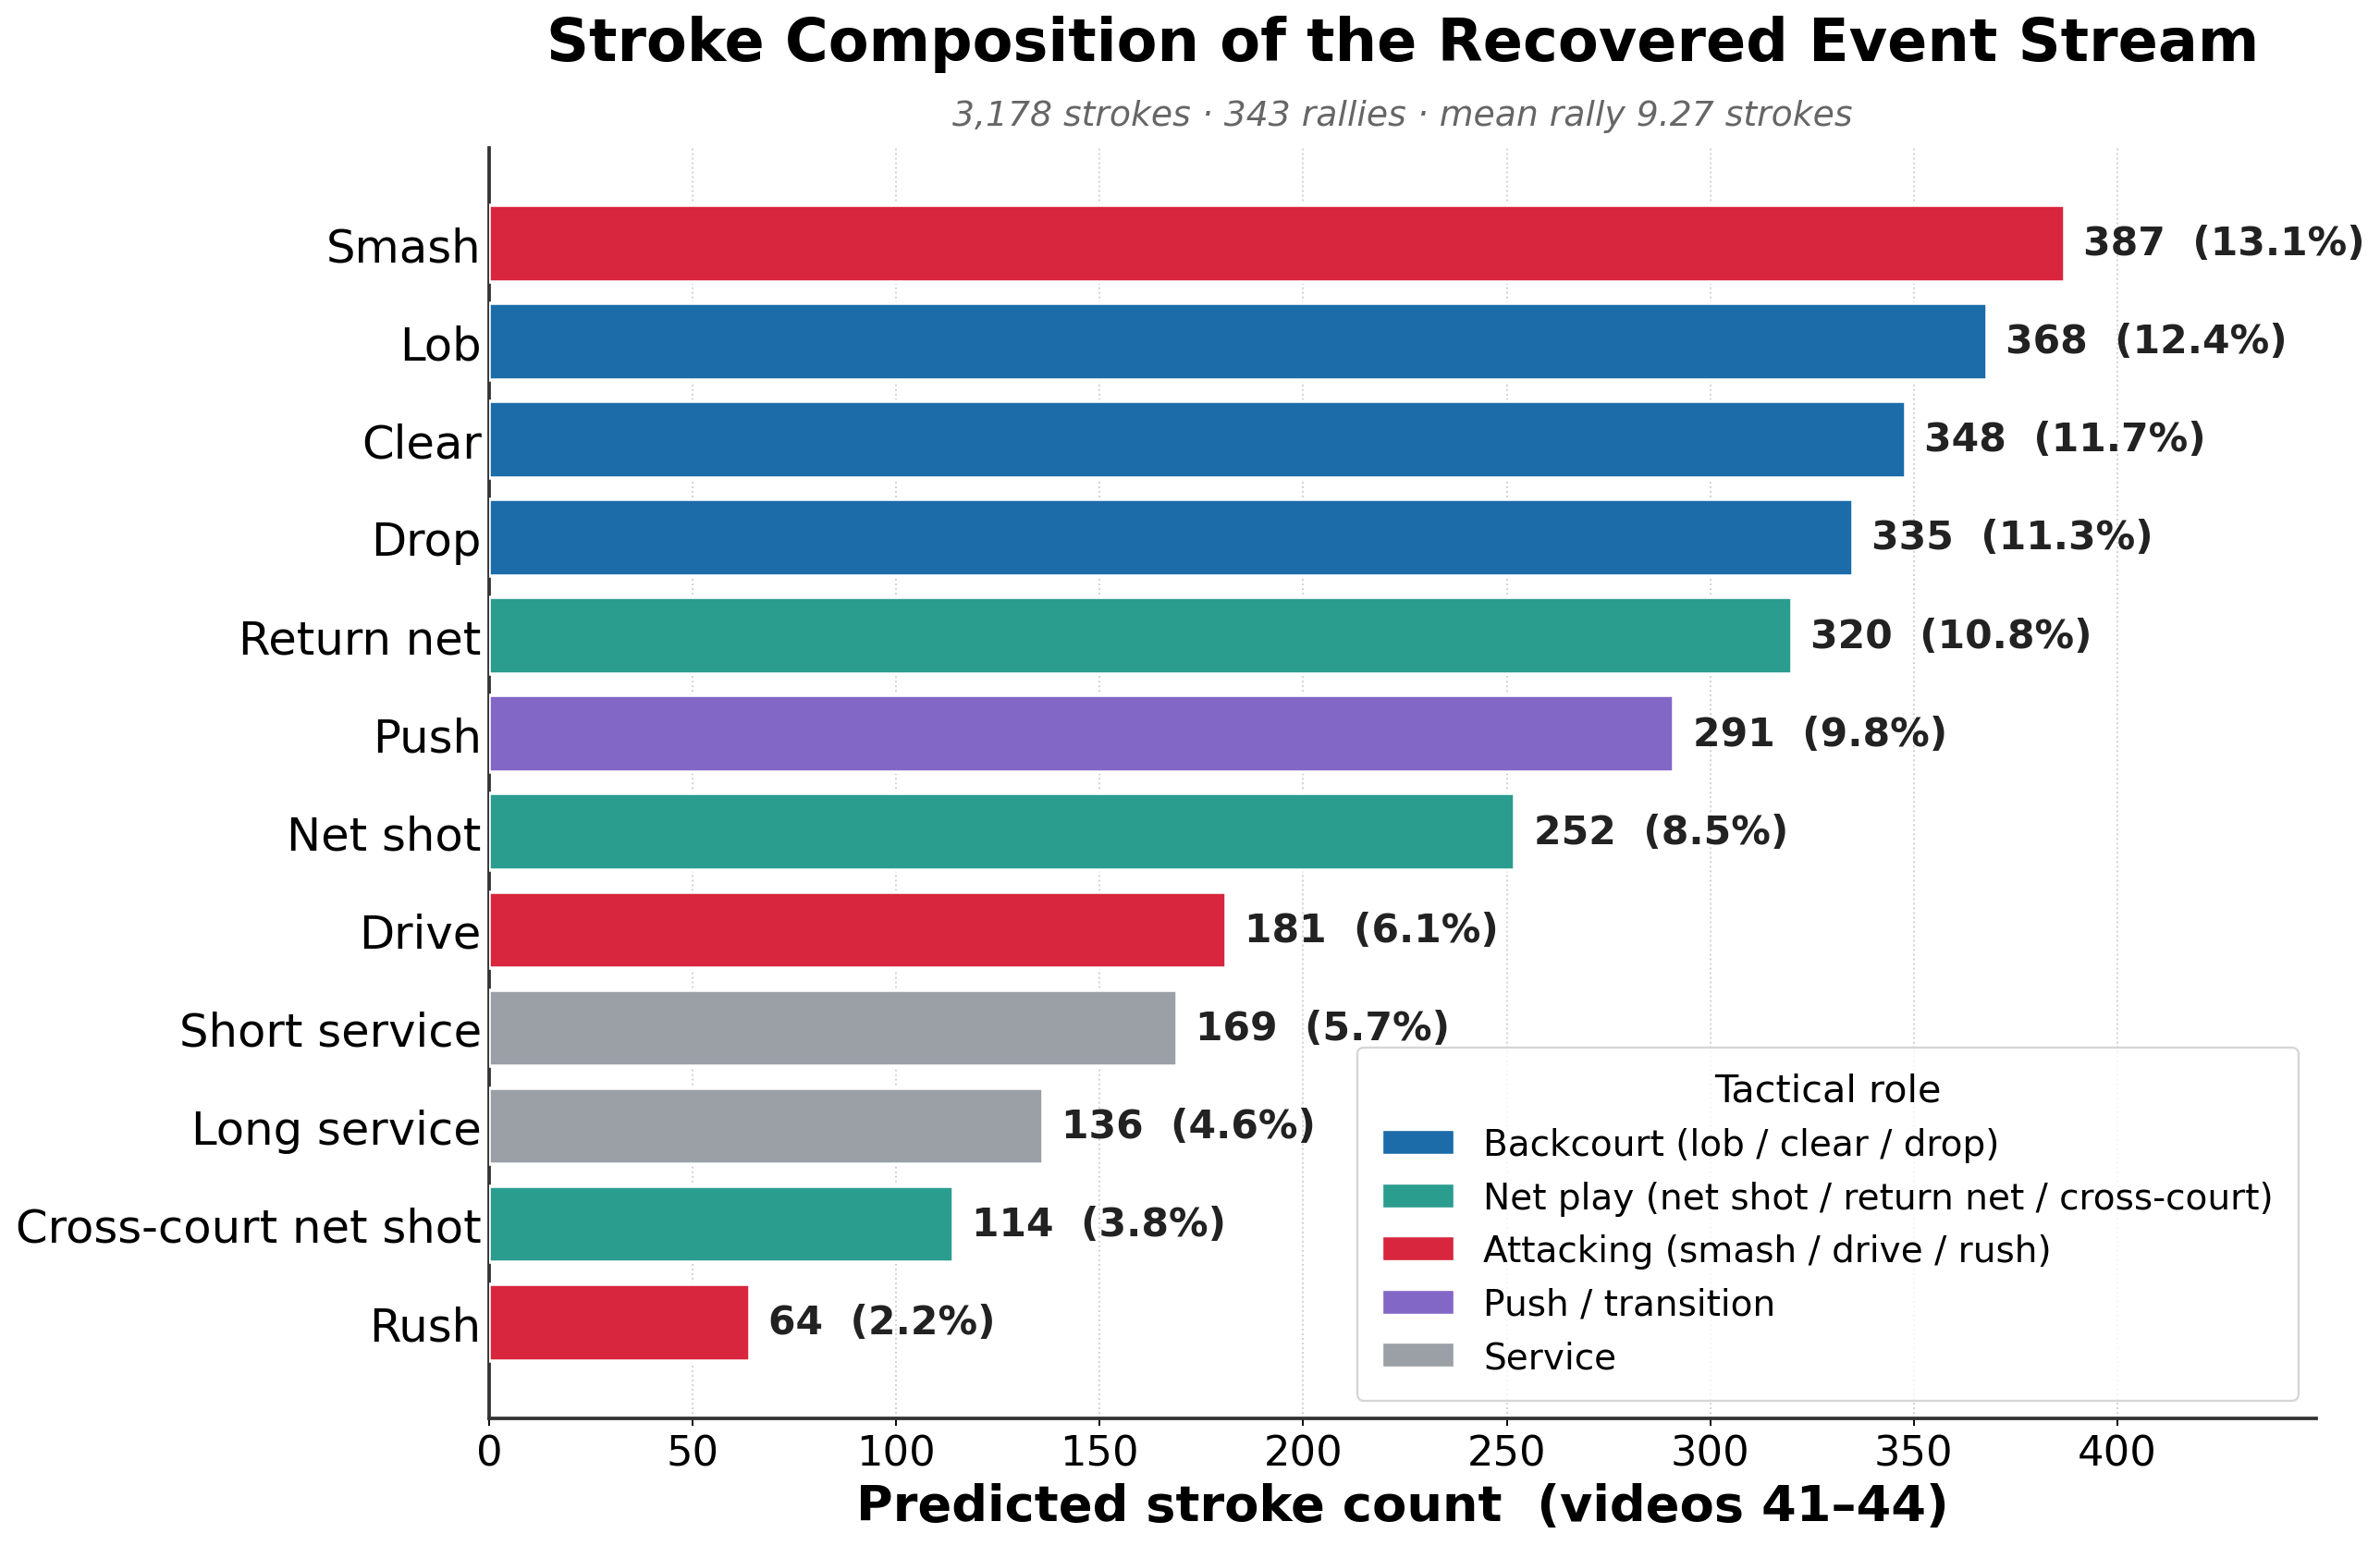
\includegraphics[width=\linewidth]{images/stroke_distribution.png}
  \caption{\textbf{Stroke composition.} Distribution of predicted stroke types (side-agnostic) across the unseen evaluation set. Smash, lob, and clear form a tight leading band, followed by drop, return net, and push, reflecting a near-even mix of attacking and rally-sustaining strokes.}
  \label{fig:stroke_distribution}
\end{figure}

\subsection{Markov Transitions}

Markov modeling converts each rally into stroke-to-stroke transitions and builds
a transition matrix whose rows index the current stroke and columns index the
next. Let $C_{ij}$ denote the number of times stroke $i$ is immediately
followed by stroke $j$ in the data; the corresponding row-normalised
transition probability is
\[
T_{ij} = \frac{C_{ij}}{\sum_k C_{ik}},
\]
which defines a first-order Markov chain over the stroke vocabulary.
This matrix answers: given a stroke, what reply tends to follow next?
To quantify how well the predicted matrix \(\hat{T}\) matches the ground
truth \(T\), we report the Frobenius norm
\(\|T - \hat{T}\|_F = \sqrt{\sum_{ij}(T_{ij} - \hat{T}_{ij})^2}\)
and the per-row Kullback--Leibler divergence
\(\mathrm{KL}(T_i \Vert \hat{T}_i) = \sum_j T_{ij} \log\frac{T_{ij}}{\hat{T}_{ij}}\).
Reducing the \texttt{none} rate from 56.43\% to 6.70\% cuts the Frobenius error
from 3.77 to 1.23 and the mean row KL from 11.55 to 0.51---roughly a $67\%$ and
$96\%$ reduction---when both pipelines are scored against the \emph{same}
3{,}178-event ground-truth reference (the earlier-pipeline caveat and its
own-reference score are detailed in Table~\ref{tab:transition_baselines}).

\paragraph{Transition baselines.}
A raw error of $1.23$ is only meaningful against a yardstick, so
Table~\ref{tab:transition_baselines} places the predicted matrix between two
naive references and an ablation baseline, all scored against the same
ground-truth transitions. The \emph{earlier pipeline} in that table is a prior
version of \method{} that used a weaker pose model and no BST fine-tuning: it
predicted the \texttt{none} class for 56.43\% of all stroke windows, meaning
more than half the rally sequence was discarded before any mining could begin.
We include it to quantify the cost of broken sequence coherence---not as a
comparison with an external system, but as an internal ablation showing how much
the \texttt{none}-reduction step is worth. A \emph{uniform-random} row-normalized matrix scores
$2.77$, and a \emph{unigram} (memoryless) model---every row set equal to the
marginal next-stroke distribution, i.e.\ ignoring the current stroke---scores
$2.61$. The current pipeline ($1.23$) more than halves both, which is the key
evidence that the recovered transitions encode genuine first-order structure
rather than merely reproducing overall stroke frequencies. By contrast, the
earlier \texttt{none}-flooded pipeline ($3.77$ on the same reference) is
\emph{worse than even the random baseline}: collapsing half of all rows onto the
\texttt{none} column
pushes the matrix further from ground truth than chance, a concrete illustration
of how broken sequence coherence destroys transition structure.

\begin{table}[t]
  \caption{Transition-recovery baselines. Frobenius and mean row-KL distance to
  the matched ground-truth transition matrix on the 3{,}178-event set (25
  side-aware states). All five rows share this single reference; the earlier
  pipeline's predicted matrix is estimated from its own 2{,}986-event run but
  compared against the identical reference (against its own matched truth it
  scores a near-identical 3.65 / 11.72). Lower is better.}
  \label{tab:transition_baselines}
  \centering
  \small
  \begin{tabular}{lrr}
    \toprule
    Transition model & Frobenius\,$\downarrow$ & Mean row KL\,$\downarrow$ \\
    \midrule
    Uniform-random rows              & 2.77 & 2.23 \\
    Unigram (memoryless)             & 2.61 & 1.58 \\
    Earlier pipeline (\texttt{none} 56.4\%) & 3.77 & 11.55 \\
    Current pipeline (\texttt{none} 6.7\%)  & \textbf{1.23} & \textbf{0.51} \\
    Ground truth (reference)         & 0.00 & 0.00 \\
    \bottomrule
  \end{tabular}
\end{table}

\paragraph{Attack--defence grammar.}
All transition probabilities below are computed from the 3{,}178 predicted
strokes across four elite matches: Ng Ka Long Angus vs.\ Kidambi Srikanth
(QF), Sindhu vs.\ Chochuwong (QF), Marin vs.\ Chochuwong (SF), and
Antonsen vs.\ Axelsen (Finals) --- all from the HSBC BWF World Tour Finals
2020. Side labels (Top/Bottom) are camera-relative; figures are reported
after pooling both sides.

\textbf{Net shot is the primary setup stroke.}
Net shots force a lob reply 52.0\% of the time and a push 20.9\%,
making them the most reliable stroke for creating an attacking opportunity
rather than winning the point directly. The remaining 20.3\% sees the
opponent answer with another net shot, initiating a net-zone exchange.

\textbf{Lob and clear both invite attacking replies, through different paths.}
After a lob, the opponent smashes 41.6\% of the time and drops 29.1\%,
with only 24.2\% answered by a clearing reply. After a clear, the split is
almost three-way: smash 35.3\%, clear-to-clear 30.6\%, and drop 30.4\%.
The clear-to-clear continuation is the predicted ``waiting game'': neither
player commits to an attack until a sufficiently weak ball arrives.
This three-way branching after a clear is a key distinction from the lob,
where the attacking smash is the dominant choice.

\textbf{Smash almost never ends the rally.}
Across the four matches, 61.9\% of smashes draw a return net (defensive
block), 11.8\% a drive, and 11.7\% a cross-court net shot. Fewer than 3\%
of smashes are followed by a lob or net shot---meaning the rally almost
always continues. The smash accumulates pressure rather than finishing
points.

\textbf{Drop opens net play.}
A drop is answered with a net shot 21.4\% of the time, a push 16.7\%, or
a cross-court net shot 11.7\%, placing roughly half of drop replies into
the net zone. This positions the dropping player to threaten with a
subsequent net attack or rush.

\textbf{Defensive return restores neutral.}
After a return net, the most common reply is a push (31.5\%) or lob (23.4\%),
resetting the rally to a neutral net-zone or backcourt exchange rather than
immediately launching another attack.

Together these five patterns form a repeating rally cycle
(Figure~\ref{fig:transition_heatmap}):
net shot $\rightarrow$ lob $\rightarrow$ smash $\rightarrow$ return net
$\rightarrow$ push/lob $\rightarrow$ net shot, punctuated by the
backcourt ``waiting'' phase (clear $\rightarrow$ clear $\rightarrow$ smash)
whenever both players retreat to consolidate position.

\begin{figure}[t]
  \centering
  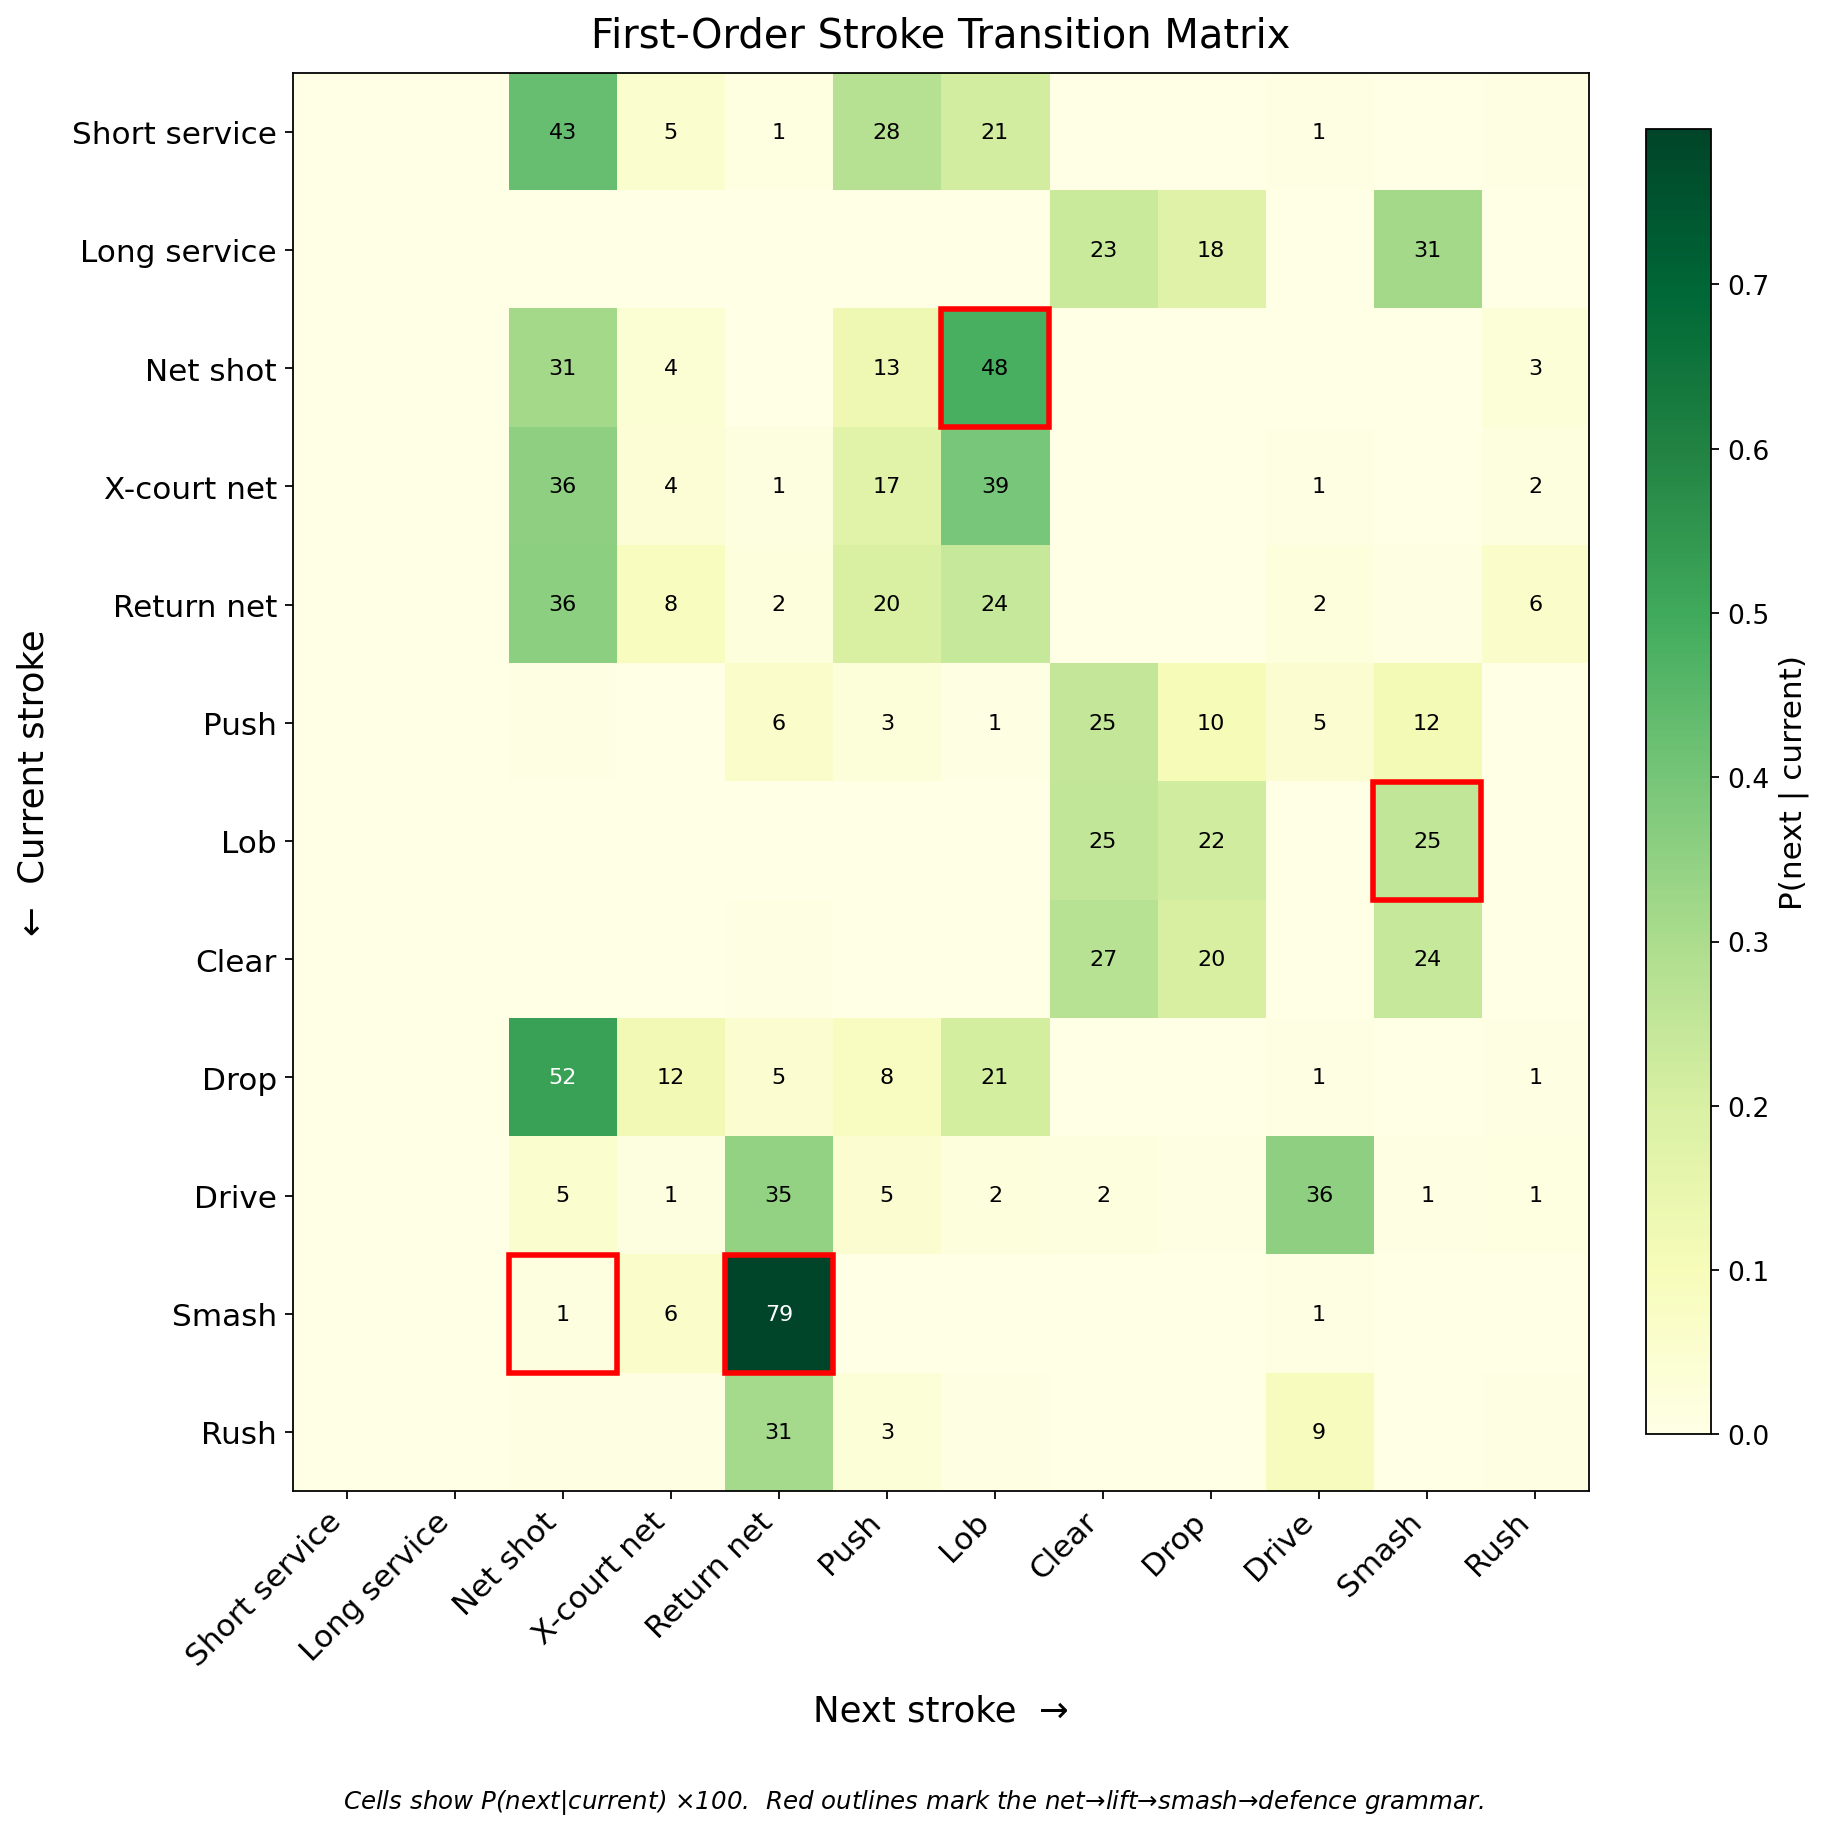
\includegraphics[width=\linewidth]{images/transition_heatmap.png}
  \caption{\textbf{Transition matrix.} First-order stroke-transition matrix
  from the predicted event stream across videos~41--44 (side-agnostic,
  \texttt{none} excluded). Each cell reports
  $P(\text{next}\mid\text{current})\times100$; rows index the current stroke
  and columns the next. Red outlines mark the recovered attack--defence
  grammar: net~$\rightarrow$~lob, lob/clear~$\rightarrow$~smash,
  smash~$\rightarrow$~return net, and clear~$\rightarrow$~clear (backcourt
  waiting exchange).}
  \label{fig:transition_heatmap}
\end{figure}

\subsection{Frequent Motif Mining}

Motif mining extends Markov analysis from single transitions to repeated
multi-stroke phrases. Contiguous $n$-grams are ranked by \emph{rally support},
defined for a motif $m$ as
\[
\mathrm{support}(m) = \frac{\#\{\text{rallies containing } m\}}{\#\{\text{total rallies}\}},
\]
the fraction of rallies that contain at least one instance of $m$.  In the
ground truth, the dominant motif is net~$\rightarrow$~lob~$\rightarrow$~smash~$\rightarrow$~defensive
reply, which appears in about 11\% of rallies. The predicted stream recovers
this structure in side-aware form: Top net~$\rightarrow$~Bottom lob~$\rightarrow$~Top
smash~$\rightarrow$~Bottom return net appears in 4.7\% of rallies, and shorter
sub-sequences are common. Motif mining thus translates the transition matrix
into an interpretable tactical phrase: net pressure induces a lift, the lift
creates attacking opportunity, and the attack draws a defensive reply.
Figure~\ref{fig:motif_support} reports the rally support of the most frequent
motifs and highlights which repeated phrases occur most reliably.

\paragraph{Validation against ground truth.}
Mining the same rallies from the matched true labels, the dominant four-stroke
phrase net~$\rightarrow$~lob~$\rightarrow$~smash~$\rightarrow$~return net occurs
in $12.2\%$ of true rallies and is recovered as the single most frequent
predicted motif ($7.1\%$ side-agnostic; $4.7\%$ in strict side-aware form). To
quantify agreement beyond the top phrase, we compare predicted and true motif
\emph{supports} across all motifs above $2\%$ rally support. The rankings agree
well at tactical-phrase scale---Spearman $\rho=0.85$ for pairs ($n{=}2$) and
$\rho=0.66$ for triples ($n{=}3$), with top-10 overlap@10 of $0.60$ and $0.70$
(Jaccard $0.43$ and $0.54$)---but degrade for four-grams ($\rho=0.32$,
overlap@10 $0.40$) as longer phrases compound per-stroke errors
(Figure~\ref{fig:mining_validation}b). The
mined tactical grammar is thus reliable at the two- and three-stroke scale that
carries most coaching value, with longer phrases interpreted more cautiously.

\begin{figure}[t]
  \centering
  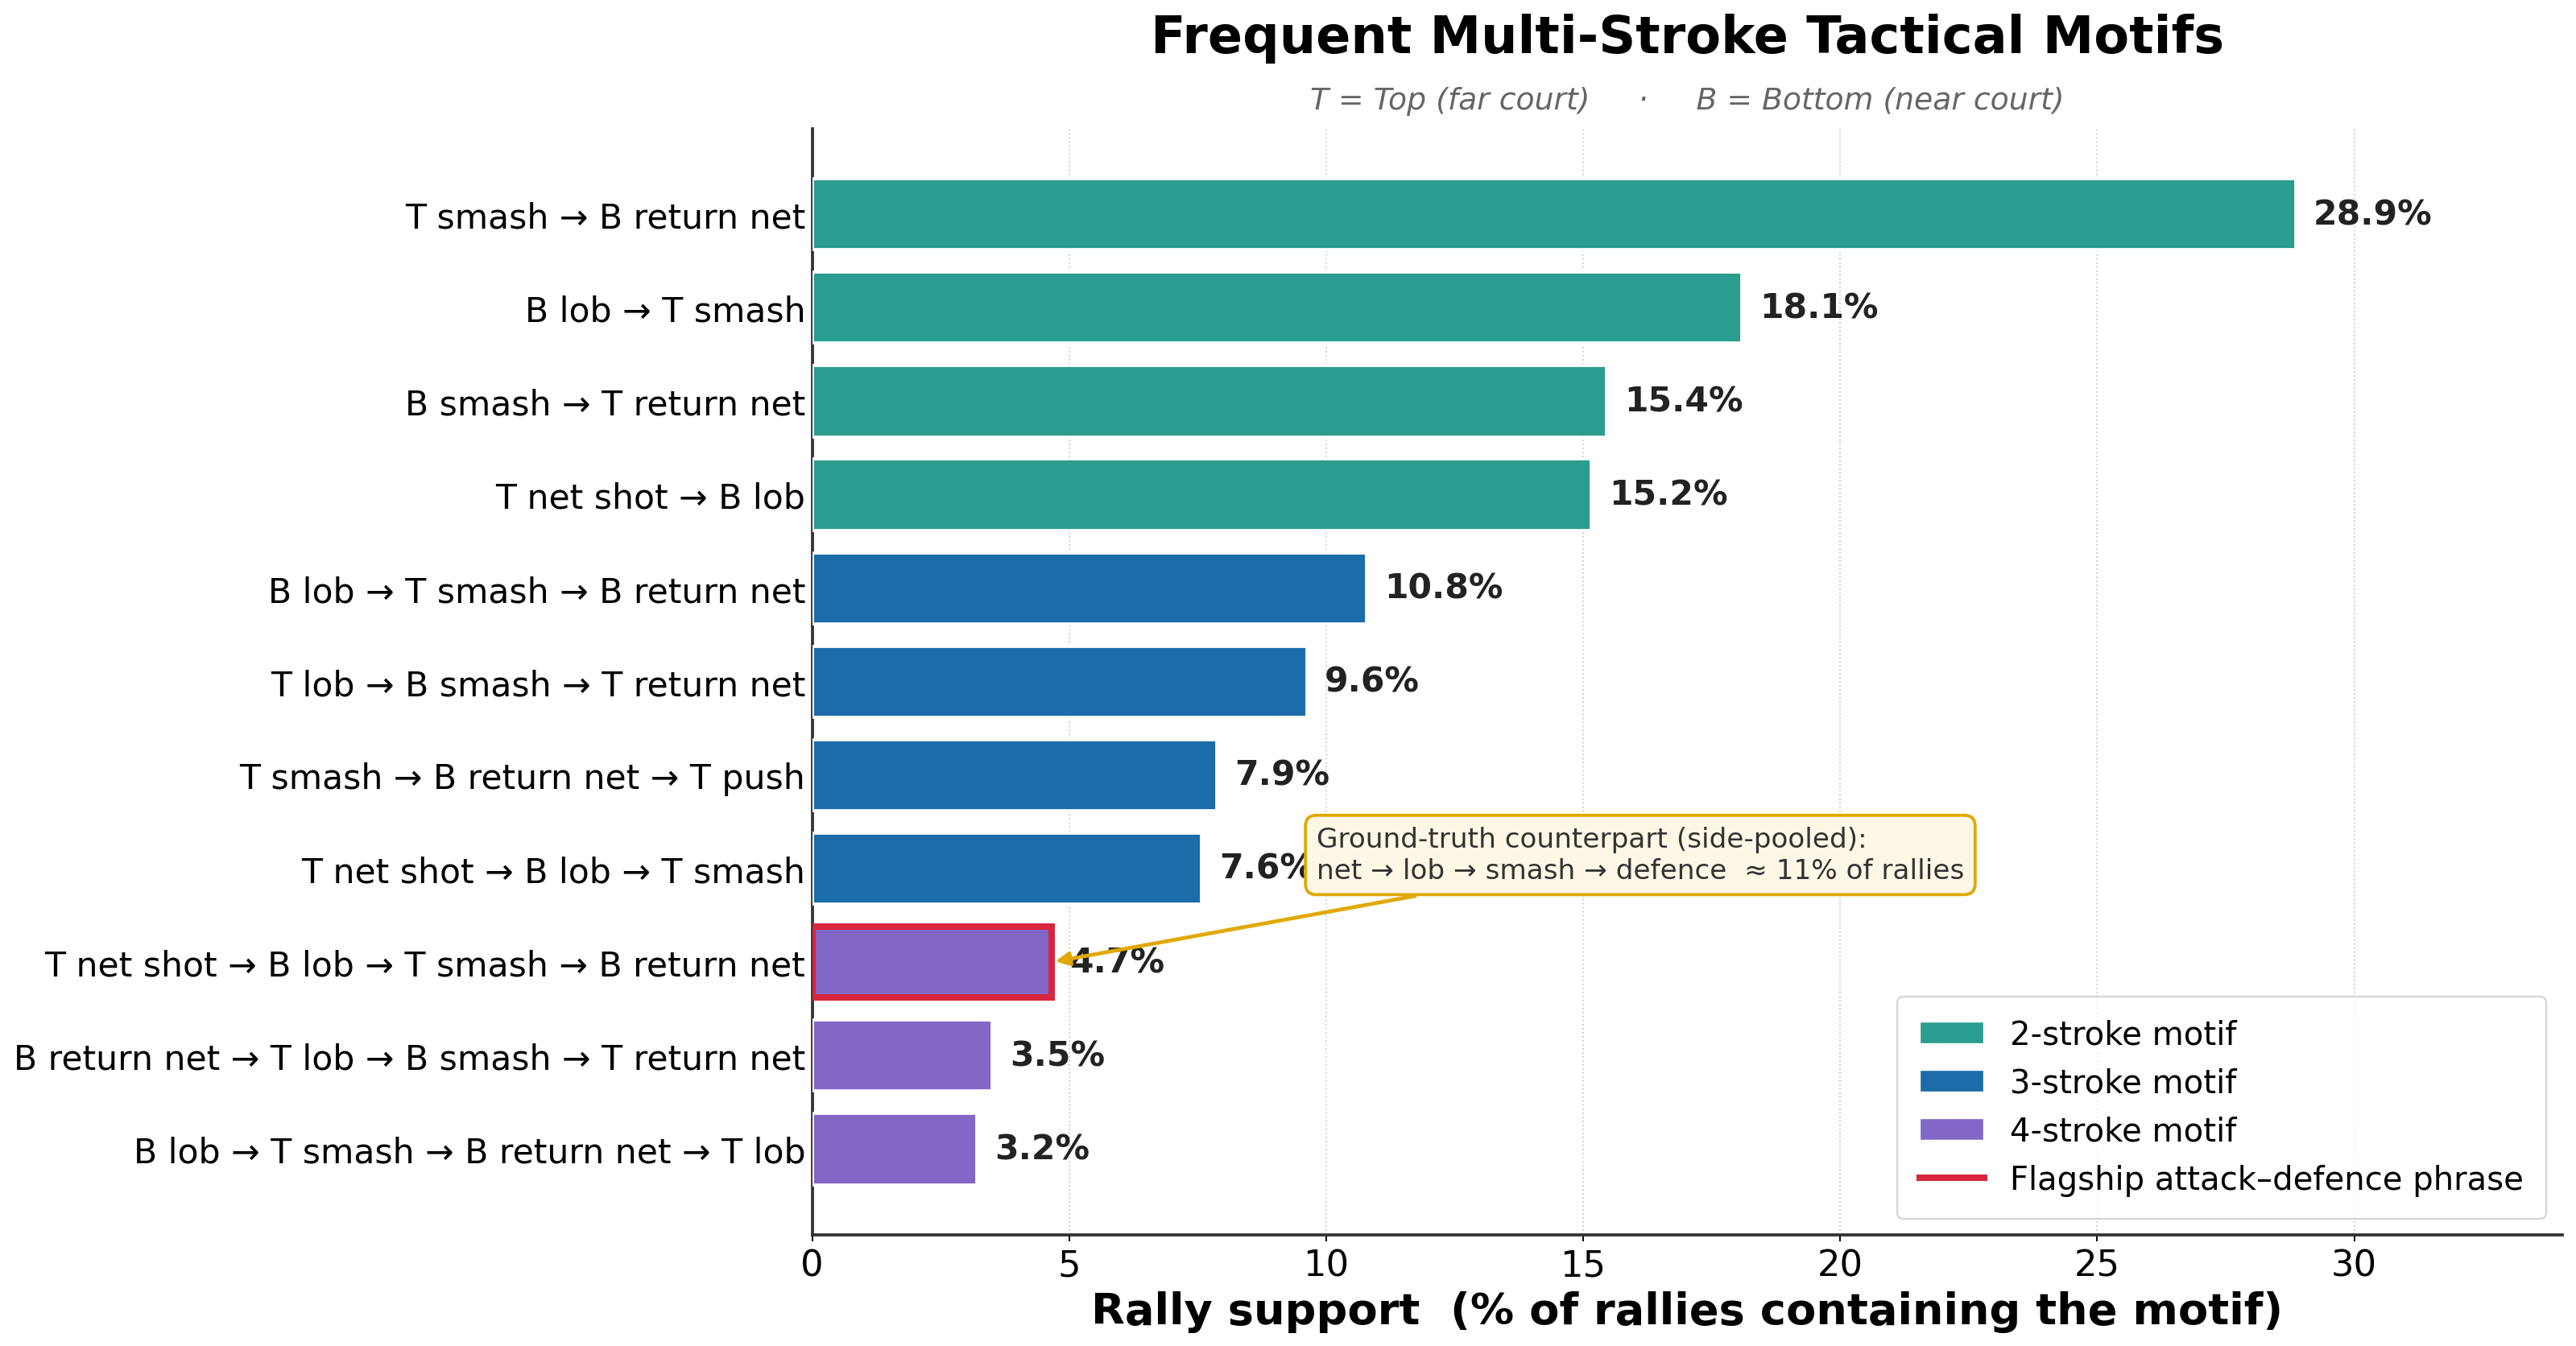
\includegraphics[width=\linewidth]{images/motif_support.png}
  \caption{\textbf{Frequent motifs.} Rally support of the most common contiguous multi-stroke motifs. Higher support indicates that the phrase appears in a larger fraction of rallies, making the repeated tactical grammar easier to interpret.}
  \label{fig:motif_support}
\end{figure}

\subsection{Movement Profiling}
Movement profiling relates spatial behaviour to stroke selection. Player
positions are projected into a player-centric normalized court frame using
ShuttleSet homographies, where $\text{forward}=1$ points toward the net and
$\text{forward}=0$ toward the baseline, so every player faces the net in the
same direction regardless of camera side. Across 2{,}300 valid events and
1{,}710 valid displacement pairs, stroke events cluster near the court centre
(Figure~\ref{fig:movement_profiling}, left), confirming the central-base
positioning expected in singles badminton.
Per-profile statistics are computed along twelve movement dimensions:
mean forward position, lateral and forward position spread, mean
inter-stroke displacement, rightward, netward, and baseline-ward displacement
rates, smash rate, net attack rate, lift/clear rate,
smash-after-large-displacement rate, and rear-court smash rate.

To quantify pairwise relationships, we compute the Pearson correlation
coefficient
\[
r = \frac{\sum_{k} (x_k - \bar{x})(y_k - \bar{y})}{\sqrt{\sum_k (x_k -
\bar{x})^2\, \sum_k (y_k - \bar{y})^2}},
\]
where $\bar{x}$ and $\bar{y}$ are sample means across profiles. Because only
$n=16$ player-set profiles enter these correlations, we report each with its
$95\%$ confidence interval and two-sided $p$-value and apply Benjamini--Hochberg
(BH) false-discovery-rate control across the full set of $\binom{12}{2}=66$
pairwise correlations from which the five below are selected; at this sample size
$|r|$ must reach roughly $0.50$ to clear raw significance. The two \emph{direct}
movement-to-attack associations do not clear it: net-ward displacement vs.\ smash
frequency is $r=+0.30$ ($95\%$ CI $[-0.23,+0.70]$, $p=0.25$) and baseline-ward
retreat vs.\ smash is $r=-0.34$ ($[-0.71,+0.19]$, $p=0.20$). Their signs match
the expected direction---forward movement preceding attack---but at $n=16$ we
treat them as \emph{suggestive, not confirmed}. The three \emph{structural}
correlations are individually significant: lateral coverage width vs.\ net-ward
frequency $r=+0.73$ ($[+0.37,+0.90]$, $p=0.001$), forward-position variability
vs.\ net-attack rate $r=+0.56$ ($[+0.09,+0.83]$, $p=0.025$), and mean forward
position vs.\ rear-court smash rate $r=-0.68$ ($[-0.88,-0.28]$, $p=0.004$). Under
the stricter full-matrix BH correction only the strongest, $r=+0.73$, retains
significance ($q=0.04$); $r=-0.68$ and $r=+0.56$ fall to $q=0.085$ and $q=0.27$,
so we report them as real but multiplicity-sensitive. The robust takeaway is
geometric---players who cover more lateral ground also press the net more
($r=+0.73$)---whereas the direct movement-to-smash link is only weakly supported
at this sample size and should be read as indicative.

\paragraph{Movement-style groups.}
Applying KMeans to the standardized 12-dimensional profiles and selecting
$k=3$ by joint silhouette and bootstrap-ARI criteria yields three distinct
movement archetypes across the 16 player-set profiles (Figure~\ref{fig:movement_clusters}).
Table~\ref{tab:movement_clusters} summarises the centroid values of the key
discriminating features.

\begin{table*}[h]
  \caption{Movement-style cluster centroids ($k=3$, silhouette 0.151, bootstrap ARI 0.365).
           Forward position: 1\,=\,net, 0\,=\,baseline. All rates are fractions.}
  \label{tab:movement_clusters}
  \centering
  \small
  \begin{tabular}{lrrr}
    \toprule
    Feature & Cluster 0 & Cluster 1 & Cluster 2 \\
            & Active Attacker & Passive Baseliner & Rear-court Dom. \\
            & ($n=8$) & ($n=3$) & ($n=5$) \\
    \midrule
    Mean forward position         & 0.482 & \textbf{0.501} & 0.379 \\
    Netward displacement rate     & \textbf{0.434} & 0.360 & 0.380 \\
    Baseline-ward displacement rate & 0.155 & 0.189 & \textbf{0.207} \\
    Smash rate                    & \textbf{0.101} & 0.064 & 0.077 \\
    Net attack rate               & 0.385 & 0.266 & \textbf{0.395} \\
    Rear-court smash rate         & 0.847 & 0.714 & \textbf{0.975} \\
    Smash after large displacement & 0.652 & 0.663 & \textbf{0.802} \\
    \bottomrule
  \end{tabular}
\end{table*}

\textbf{Cluster~0 --- Active Attacker} ($n=8$, majority): Mid-court base
($\mu_\text{fwd}=0.482$) with the highest net-ward movement rate (0.434),
the highest smash rate (10.1\%), and the highest net attack rate (38.5\%).
These player-sets actively press the net and create attacking opportunities
via overhead smashes and net pressure, representing the dominant all-round
aggressive style across the matches.

\textbf{Cluster~1 --- Passive Baseliner} ($n=3$): Despite having the most
net-forward average position ($\mu_\text{fwd}=0.501$), these profiles show
the lowest net-ward displacement rate (0.360), lowest smash rate (6.4\%), and
lowest net attack rate (26.6\%). The apparent contradiction---positioned close
to the net yet generating the fewest net attacks---suggests reactive, defensive
positioning: these players are pushed toward the net by their opponent rather
than choosing to attack it. The lowest rear-court smash rate (71.4\%) also
reflects fewer committed overhead situations.

\textbf{Cluster~2 --- Rear-court Dominator} ($n=5$): The deepest court base
($\mu_\text{fwd}=0.379$) combined with a 97.5\% rear-court smash rate tells a
coherent story: these player-sets almost exclusively smash from behind
mid-court and frequently require a large displacement to reach the shuttle
first (smash-after-large-displacement rate 80.2\%). Despite their deep base,
they also post a high net attack rate (39.5\%), pointing to full-court
coverage---retreating for overhead power, then pressing forward for net
exchanges.

\paragraph{Validation against ground truth.}
Because these archetypes are built from \emph{predicted} stroke rates, we test
how much they depend on classifier error by re-deriving the identical 16
profiles from ground-truth labels (the positional features are
label-independent, so only the five stroke-rate axes change). The predicted
stroke-rate features track their true counterparts closely across profiles, with
per-feature Pearson correlations of $0.74$--$0.84$ (mean $\bar{r}=0.79$;
Figure~\ref{fig:mining_validation}d), so the \emph{profile axes themselves are
faithful}. The discrete cluster assignment is the weaker link: the
predicted-derived and truth-derived $k{=}3$ partitions agree at an adjusted Rand
index of $0.17$ (versus $\approx0.00$ expected for random labels). This
predicted-vs-truth \emph{agreement} ARI is distinct from---and lower than---the
bootstrap \emph{stability} ARI of $0.365$ reported above, and it sits within the
noise band expected when partitioning only 16 units. We therefore present the
three movement archetypes as a descriptive summary of playing style rather than
a stable, transferable player taxonomy.

\begin{figure*}[t]
  \centering
  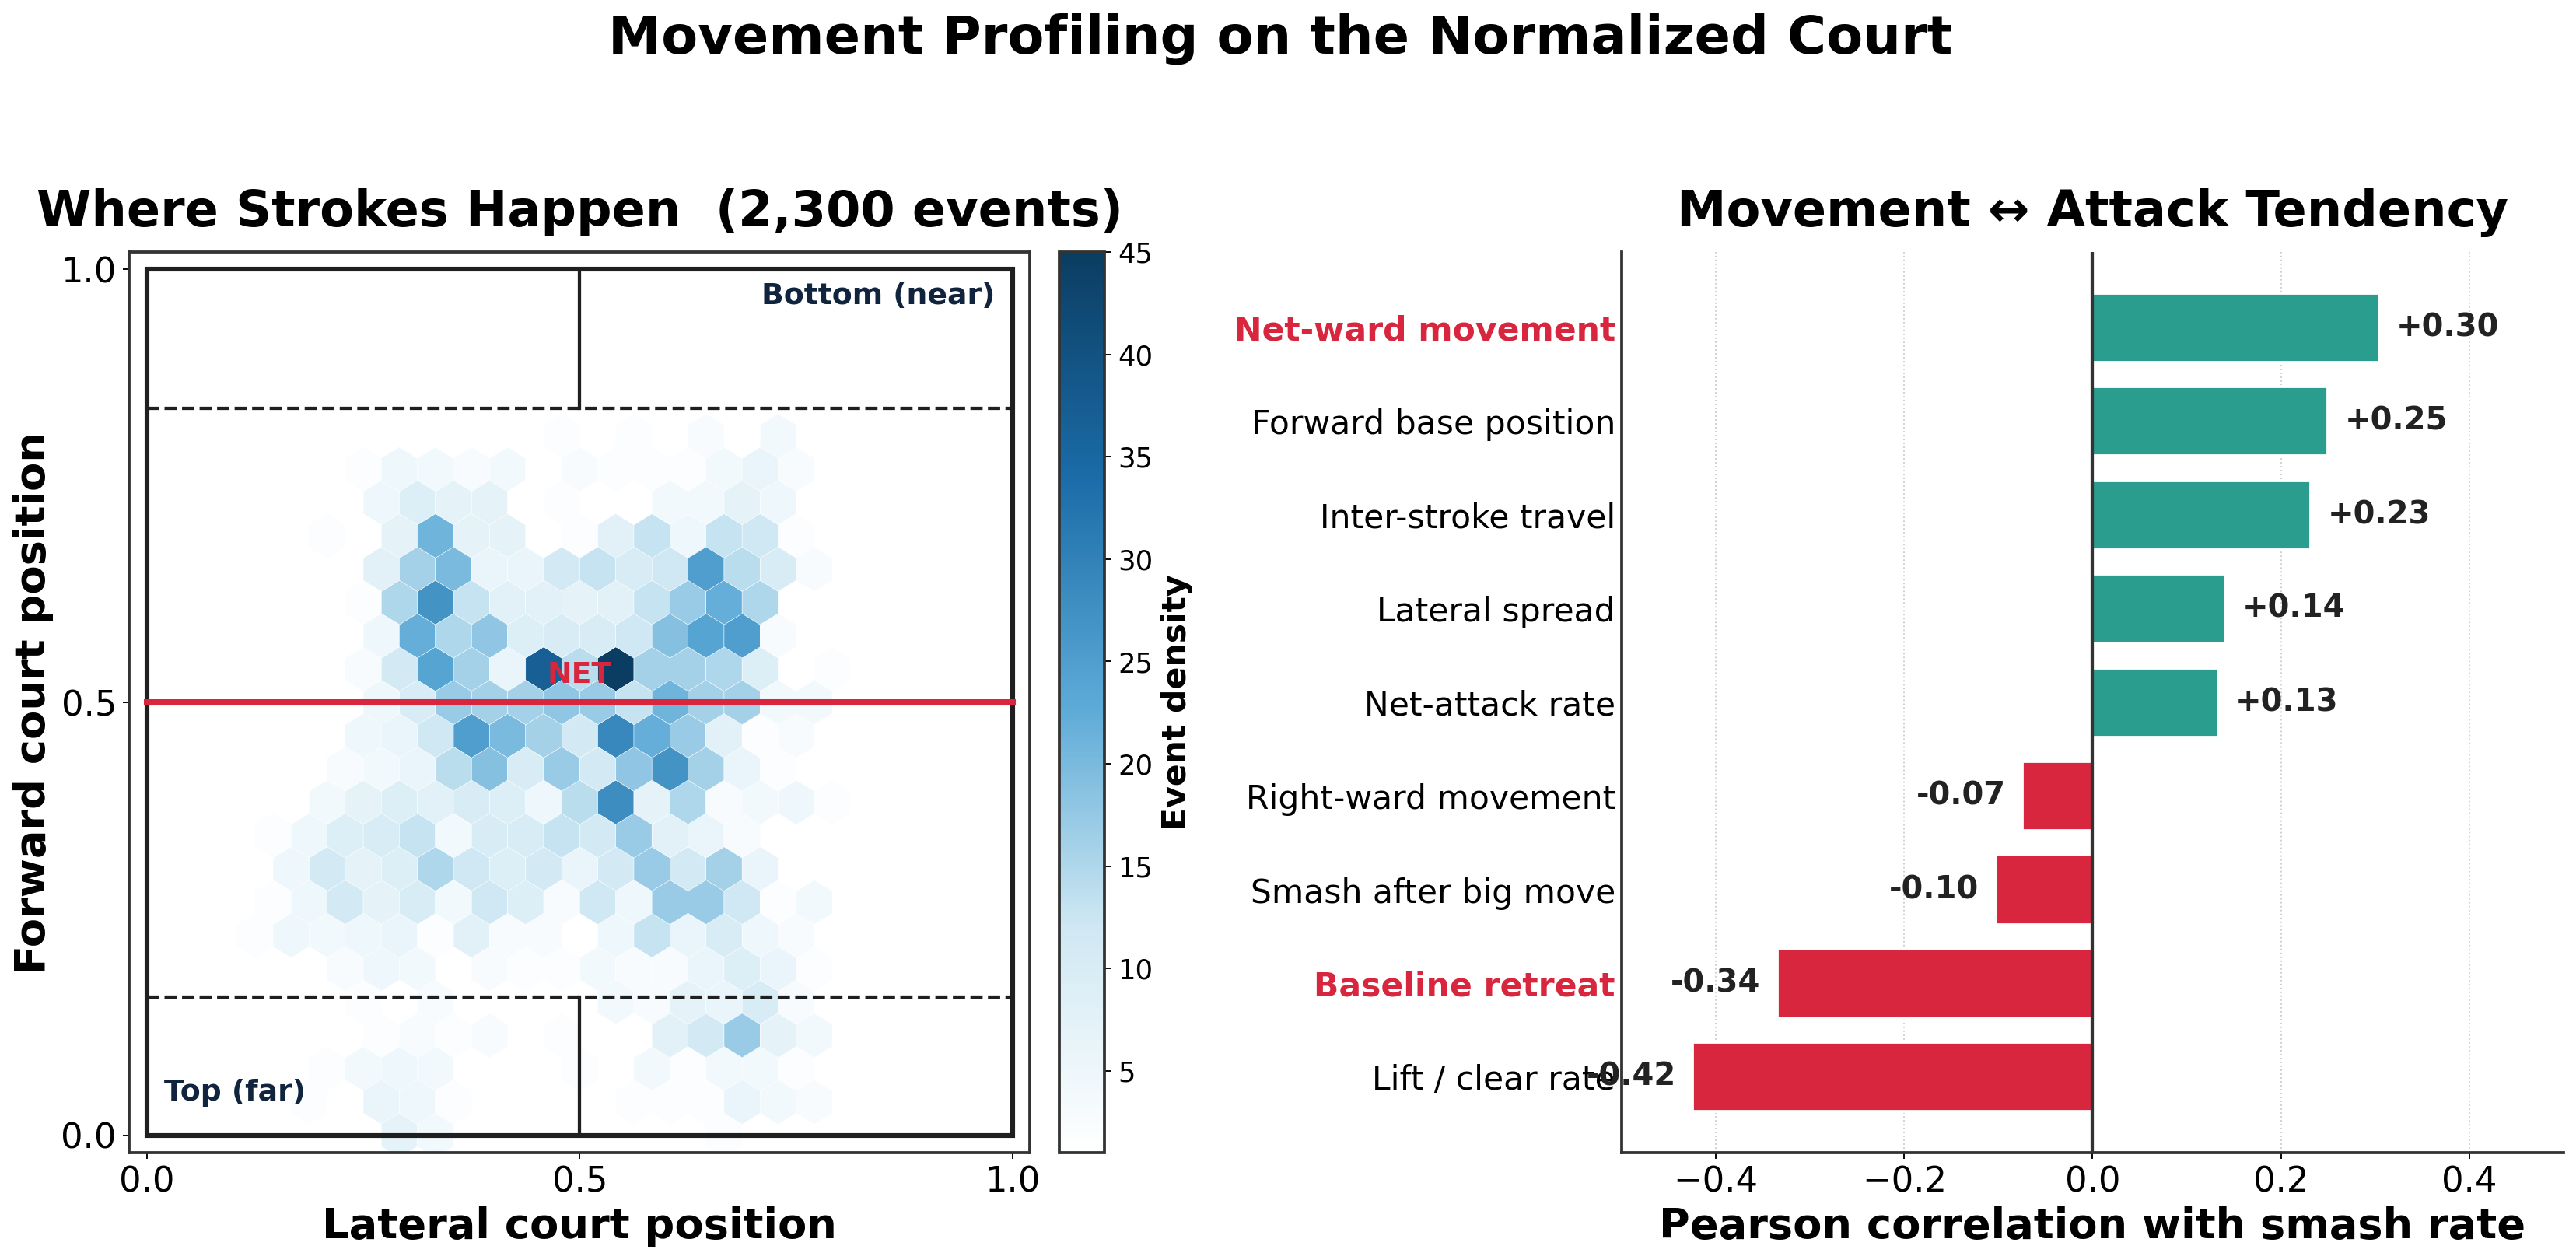
\includegraphics[width=\linewidth]{images/movement_profiling.png}
  \caption{\textbf{Movement profiling.} \emph{Left:} occupancy of 2{,}300
  stroke events on the normalized court, showing the central-base tendency.
  \emph{Right:} Pearson correlation of movement features with smash rate.
  Net-ward movement ($r=+0.30$) and baseline retreat ($r=-0.34$) point in the
  expected directions but are not significant at $n=16$ ($p>0.2$); the
  significant structural correlation is lateral coverage vs.\ net-ward frequency
  ($r=+0.73$, $p=0.001$, inter-feature, not shown here).}
  \label{fig:movement_profiling}
\end{figure*}

\begin{figure}[t]
  \centering
  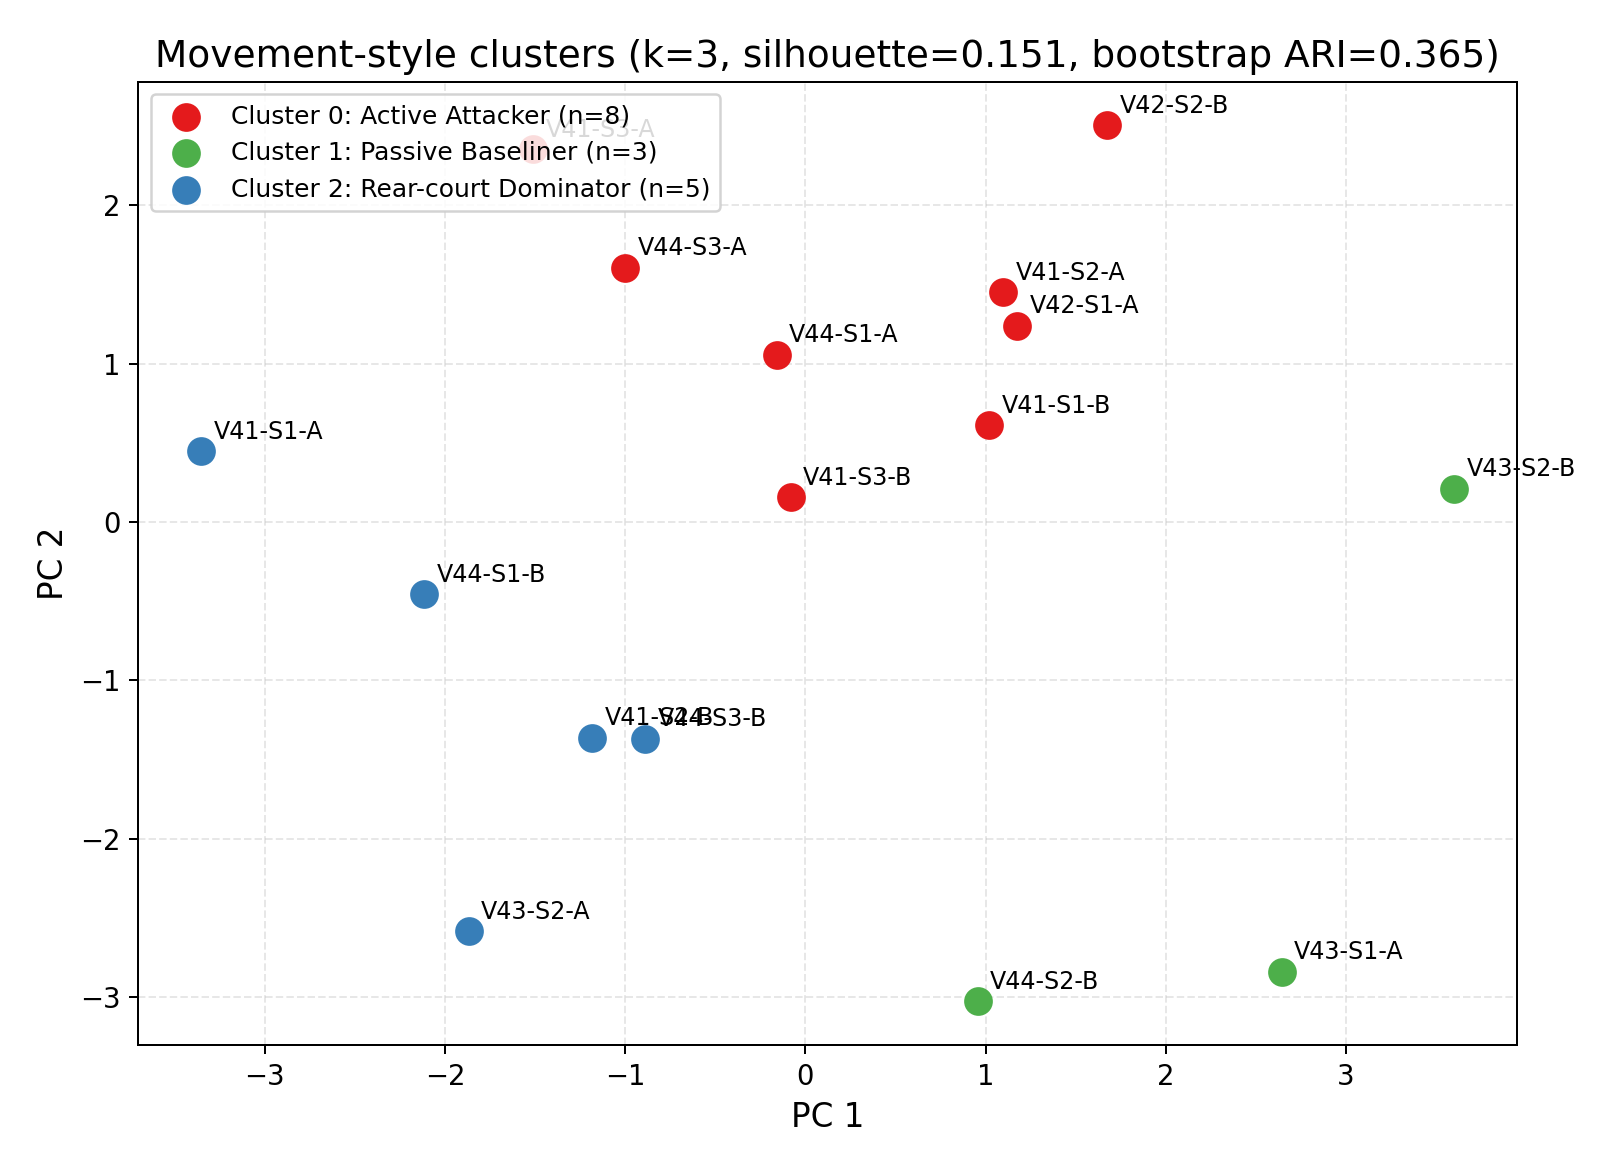
\includegraphics[width=\linewidth]{images/movement_clusters.png}
  \caption{\textbf{Movement-style clusters.} PCA projection of 16 player-set
  profiles ($k=3$, silhouette 0.151, bootstrap ARI 0.365), labelled by
  video, set, and player (A/B). \textbf{Cluster~0} (red) groups active
  attackers with the highest net-ward movement and smash rates;
  \textbf{Cluster~1} (green) groups passive baseliners with low attack rates
  despite a net-forward position; \textbf{Cluster~2} (blue) groups
  rear-court dominators who almost exclusively smash from behind mid-court
  after large displacements.}
  \label{fig:movement_clusters}
\end{figure}

\subsection{Mining Validation}

Strong perception metrics do not by themselves establish that the mined tactics
are correct: a classifier could score well per stroke yet still distort
aggregate statistics. We therefore close the loop by running each analysis on
both the predicted and the matched ground-truth labels and reporting the gap,
summarized in Table~\ref{tab:mining_eval} and visualized in
Figure~\ref{fig:mining_validation}. Four of the five views survive end-to-end
prediction well. Stroke composition stays close to truth ($\mathrm{KL}=0.04$,
$4\times$ better than uniform); the transition matrix ($\mathrm{Frobenius}=1.23$)
clearly beats both the unigram ($2.61$) and uniform-random ($2.77$) baselines,
showing that real first-order structure is recovered; and motif support rankings
correlate strongly with truth at the two- and three-stroke scale (Spearman
$0.85$ and $0.66$). The fifth view, strategy clustering, is faithful at the
feature level (mean Pearson $0.79$ between predicted- and truth-derived profiles)
but unstable at the discrete-assignment level (agreement ARI $0.17$). The overall
verdict is therefore quantitative and specific: sequence-level mining of the
predicted event stream is reliable, and the single weakest component is discrete
player clustering---not the recovered tactical grammar.

\begin{figure*}[t]
  \centering
  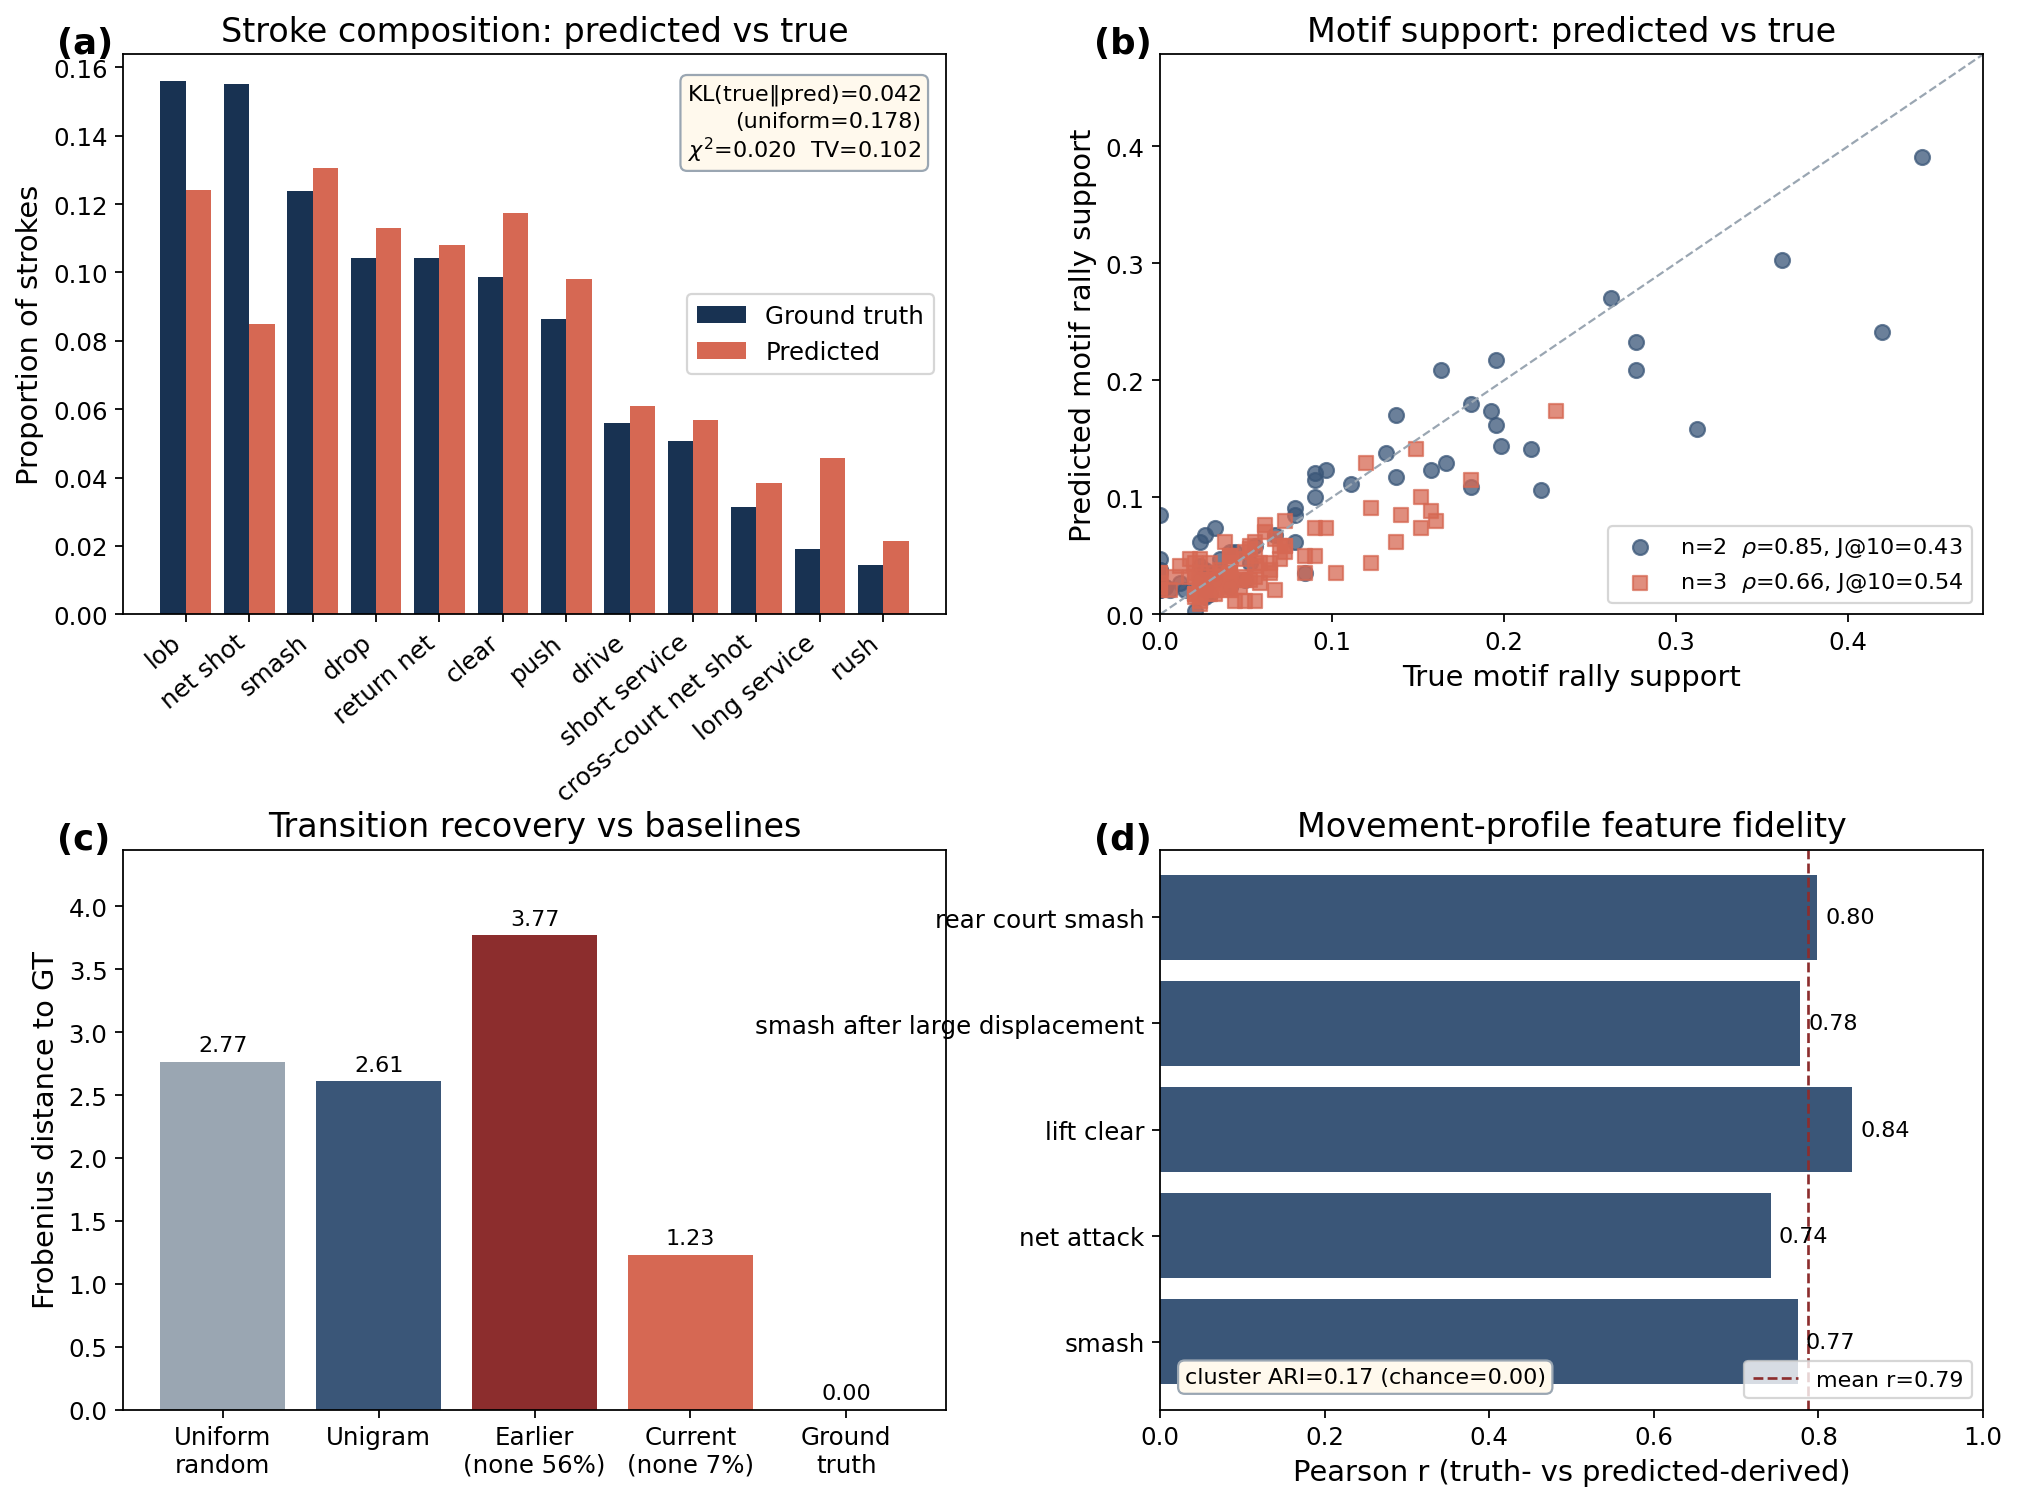
\includegraphics[width=\textwidth]{images/mining_validation.png}
  \caption{\textbf{Mining validation: predicted vs.\ ground truth on the same
  3{,}178 events.} \emph{(a)} Predicted and true stroke-type distributions stay
  close in aggregate ($\mathrm{KL}=0.04$, TV$=0.10$), though the classifier
  under-recalls net shot and lob, promoting smash to the nominal top of the
  predicted ranking. \emph{(b)} Predicted vs.\ true
  motif rally support (pairs and triples); points hug the diagonal (Spearman
  $0.85$/$0.66$), with four-gram agreement weaker ($\rho=0.32$, reported in
  text). \emph{(c)} Transition-matrix
  Frobenius distance to ground truth (all on the shared 3{,}178-event reference):
  the current pipeline ($1.23$) beats the unigram ($2.61$) and uniform-random
  ($2.77$) baselines, while the earlier \texttt{none}-flooded pipeline ($3.77$)
  is worse than chance. \emph{(d)}
  Movement-profile feature fidelity: predicted stroke-rate features correlate
  $0.74$--$0.84$ with their truth-derived values, though the discrete cluster
  agreement (ARI $0.17$) is weak.}
  \label{fig:mining_validation}
\end{figure*}

%-----------------------------------------------------------------------
\section{Discussion}
%-----------------------------------------------------------------------

The headline 69.04\% top-1 accuracy is encouraging, but accuracy is not the
result that matters most here. The decisive change is sequential: earlier
versions of the pipeline labelled over half of all windows \texttt{none},
shredding the shot-to-shot grammar, whereas improved pose features and
classifier fine-tuning cut the \texttt{none} rate to 6.70\% and make the rally
continuous again. Only on a continuous stream do the mining views become
legible and---per the validation protocol
(Table~\ref{tab:mining_eval})---demonstrably faithful rather than merely
plausible. We therefore spend this
section reading the recovered grammar the way a coach would: granting that the
numbers are trustworthy, what do they actually say about how elite singles
points are built?

\textbf{The point is built, not struck---the smash is pressure, not a finisher.}
The most counter-intuitive finding is that at this level the smash almost never
ends the rally: 61.9\% of smashes come straight back as a defensive return net,
with fewer than 3\% drawing a lob or net-shot reply---the rally continues in
almost every case. Elite
defence is good enough that one smash rarely beats it, so the smash functions to
\emph{extract} a weak reply that sets up the next stroke rather than to finish
outright. The natural tactical unit is thus the sequence
smash~$\rightarrow$~block~$\rightarrow$~kill, not the smash in isolation---which
is also why a method that preserves sequence coherence, not just per-stroke
accuracy, is the right instrument for studying the sport. For practitioners this
argues for drilling the smash-and-follow-up and valuing recovery speed after
smashing as highly as raw smash power.

\textbf{Attacks are manufactured at the net, not generated by power.}
The grammar locates the origin of attack in the forecourt. Net shots force a
lift 52.0\% of the time (and a push 20.9\%), and a lift is then answered with a
smash or drop 70.7\% of the time; drops likewise route about half of all replies
back into the net zone. The chain that ends in a smash therefore usually
\emph{begins} with a tight net shot or drop that compels the opponent to lift.
Power closes the phrase, but net skill opens it, so winning the net exchange is
the precondition for ever getting to attack.

\textbf{The lift is a concession: net play is a contest over who lifts first.}
Because lifting hands initiative away (lob~$\rightarrow$~smash 41.6\%,
lob~$\rightarrow$~drop 29.1\%), the forecourt exchange is effectively a duel to
\emph{avoid} lifting: 20.3\% of net shots draw another net shot, sustaining a
net-zone standoff in which each player tries to force the other up first. This
recasts the net not as a place to score but as a place not to concede, and
explains the premium elite players place on tight, spinning net shots.

\textbf{Elite singles runs in two gears---aggressive engagement and a patient
waiting game.} The transitions expose two stable cycles rather than one. The
engagement loop net~$\rightarrow$~lob~$\rightarrow$~smash~$\rightarrow$~return
net~$\rightarrow$~push/lob is the attacking rhythm; the clear~$\rightarrow$~clear
continuation (30.6\%) is a backcourt holding pattern in which neither player
commits until a weak ball arrives. The game is an alternation between escalation
and patience, and the discipline to keep a rally neutral---rather than forcing a
low-percentage attack from a balanced position---emerges here as a measurable
trait rather than a vague virtue.

\textbf{Mobility is a prerequisite for aggression, not a separate trait.}
The one movement correlation that survives strict multiplicity control links
lateral coverage width to net-ward pressure ($r=+0.73$, $q=0.04$): the
player-sets that cover the most sideways ground are also the ones that press the
net most. Attacking forecourt play appears to be \emph{enabled by} footwork and
court coverage---one can only commit forward while trusting the sideways
recovery---so conditioning and tactics are entangled rather than independent.

\textbf{Most elite player-sets are all-round aggressors; sustained defence is
rare and looks imposed.} Clustering separates an Active-Attacker majority
($8/16$, highest smash and net-attack rates) from a small Passive-Baseliner
group ($3/16$) and a Rear-court-Dominator group ($5/16$) that retrieves deep and
then presses forward. Tellingly, the Passive Baseliners sit \emph{closest} to
the net on average yet attack it \emph{least}: their forward position is pushed
onto them by the opponent rather than chosen, suggesting that at this level
prolonged passivity is something that happens \emph{to} a player, not a strategy
a player selects. We read these archetypes as descriptive (assignment ARI
$0.17$) rather than a transferable taxonomy, but the feature axes beneath them
are faithful ($\bar{r}=0.79$).

\textbf{The far-side bottleneck.}
Feature quality explains most of the residual error. Far-side pose is valid in
only 54.29\% of windows against 98.96\% near side; windows above 75\% far-side
validity reach 76.71\% accuracy versus 56.05\% below 50\%---a gap of more than 20
percentage points that pinpoints far-side extraction as the highest-value target
for future work. Reassuringly, the tactical conclusions above survive this
noise: the predicted-vs-true gap is smallest exactly at the two- and
three-stroke phrase scale that carries the most coaching value, so the grammar
we read off the predicted stream is the part the pipeline recovers best.


%-----------------------------------------------------------------------
\section{Limitations and Future Work}
%-----------------------------------------------------------------------

\paragraph{Benchmark scope.}
Our evaluation processes raw frames through shuttle tracking, pose extraction,
feature construction, and stroke classification. However, stroke windows still
use ground-truth hit-frame indices and court normalization relies on provided
homographies. The system should therefore be viewed as a raw-feature and
stroke-classification pipeline under supplied temporal and spatial metadata, not
a fully automatic system for arbitrary unlabeled broadcasts.

\paragraph{Perception quality.}
The main error source is far-side pose quality: its validity is just 54.29\%.
Rally filtering occasionally retains post-rally broadcast content, adding noise
near rally endpoints. Future work should focus on improving far-side detection,
tightening rally boundaries, and adopting trajectory-based hit detection to
remove reliance on annotated hit frames.

\paragraph{Output scope.}
We do not yet predict point winners, shuttle landing positions, persistent
player identities, or continuous footwork trajectories. Side-specific
distributions and clusters are therefore descriptive rather than causal: Top
and Bottom are camera-relative positions, not persistent athletes, so any side
differences reflect court geometry rather than player identity. Extending the
system to predict outcomes and integrate point-level context is a promising
direction.

\paragraph{Future work.}
Future extensions should improve far-side pose detection, replace ground-truth
hit frames with trajectory-based hit detection, automate court calibration, and
refine fine-grained stroke classification. Integrating the system with VR-based
visual analytics such as VIRD \cite{vird2023} could also provide practitioners
with interactive exploration of automatically derived event streams.

\section*{Contribution Declaration}

\begin{table}[h]
  \centering\small
  \setlength{\tabcolsep}{5pt}
  \renewcommand{\arraystretch}{1.2}
  \caption*{\textbf{Individual Contribution Split (\%)}}
  \begin{tabular}{lccc}
    \toprule
    \textbf{Task} & \textbf{Dang} & \textbf{Hieu (pd)} & \textbf{Hieu (pm)} \\
    \midrule
    Data preparation         & 20 & 50 & 30 \\
    Model integration        & 40 & 35 & 25 \\
    Experimentation          & 30 & 40 & 30 \\
    Tactical analysis        & 55 & 15 & 30 \\
    Visualisation            & 25 & 20 & 55 \\
    Manuscript writing       & 35 & 35 & 30 \\
    \midrule
    \textbf{Overall}         & \textbf{34} & \textbf{33} & \textbf{33} \\
    \bottomrule
  \end{tabular}
\end{table}

\section{Conclusion}

We presented \method, an integrated badminton video analytics and data-mining
system linking rally filtering, shuttle tracking, player pose extraction,
court-normalized feature construction, stroke classification, and five
interpretable mining analyses. On unseen ShuttleSet videos~41--44, the clean
evaluation achieves 69.04\% side-aware top-1 accuracy and 87.89\% top-3
accuracy (top-3 measures whether the correct stroke falls within the
model's three highest-scoring classes, a relevant threshold because the
dominant errors involve tactically adjacent strokes---net shot, return
net, and push---that are visually similar and occupy the same forecourt
zone). More importantly, the predicted \texttt{none} rate falls to 6.70\%
and transition-matrix error decreases substantially relative to earlier
baselines, allowing the recovered stroke stream to capture a coherent
attack–defence grammar of net pressure, forced lifts, attacking smashes, and
defensive replies. The five analyses—distributions, transitions, motifs,
movement profiles, and clustering—provide complementary evidence that the
pipeline produces a readable tactical narrative from raw video. The clearest
path forward is to improve far-side player detection and automate the steps
currently supplied by annotations.

\bibliographystyle{plain}
\bibliography{reference}


\end{document}
